\newcommand{\goodcd}{
\includegraphics[width=15mm]{icons/good-cd.png}}
\newcommand{\badcd}{
\includegraphics[width=16mm]{icons/bad-cd.png}}
\newcommand{\badcdone}{
\includegraphics[width=19mm]{icons/bad-cd1.png}}
\newcommand{\goodimage}{
\includegraphics[width=13mm]{icons/good-image.png}}
\newcommand{\goodimagetwo}{
\includegraphics[width=13mm]{icons/good-image2.png}}
\newcommand{\badimage}{
\includegraphics[width=15mm]{icons/bad-image.png}}
\newcommand{\oldcd}{
\includegraphics[width=15mm]{icons/old-cd.png}}
\newcommand{\oldimage}{
\includegraphics[width=15mm]{icons/old-image.png}}
\newcommand{\augmentedcd}{
\includegraphics[width=15mm]{icons/augmented-cd.png}}
\newcommand{\eccfile}{
\includegraphics[width=13mm]{icons/ecc-file.png}}
\newcommand{\backupone}{
\includegraphics[width=18mm]{icons/backup1.png}}
\newcommand{\backuptwo}{
\includegraphics[width=19mm]{icons/backup2.png}}
\newcommand{\rightarr}{
\includegraphics[width=11mm]{icons/right-arrow.png}}
\newcommand{\downarr}{
\includegraphics[height=11mm]{icons/down-arrow.png}}
\newcommand{\downforkarr}{
\includegraphics[height=11mm]{icons/down-fork-arrow.png}}
\newcommand{\rdiagarr}{
\includegraphics[height=9mm]{icons/rdiag-arrow.png}}
\newcommand{\ldiagarr}{
\includegraphics[height=9mm]{icons/ldiag-arrow.png}}
\newcommand{\joinarr}{
\includegraphics[height=11mm]{icons/join-arrow.png}}

\newcommand{\slotin}{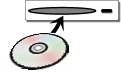
\includegraphics[height=17mm]{icons/slot-in.png}}
\newcommand{\filemanager}{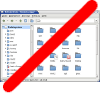
\includegraphics[height=20mm]{icons/filemanager.png}}
\newcommand{\selectdrive}{
\includegraphics[height=10mm]{icons/select-drive.png}}
\newcommand{\selectimage}{
\includegraphics[height=8.5mm]{icons/select-image.png}}
\newcommand{\selectecc}{
\includegraphics[height=8.5mm]{icons/select-ecc.png}}
\newcommand{\scanicon}{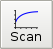
\includegraphics[height=13mm]{icons/scan-icon.png}}
\newcommand{\readicon}{
\includegraphics[height=13mm]{icons/read-icon.png}}
\newcommand{\createicon}{
\includegraphics[height=13mm]{icons/create-icon.png}}
\newcommand{\fixicon}{
\includegraphics[height=13mm]{icons/fix-icon.png}}
\newcommand{\verifyicon}{
\includegraphics[height=13mm]{icons/verify-icon.png}}
\newcommand{\stopicon}{
\includegraphics[height=13mm]{icons/stop-icon.png}}
\newcommand{\logicon}{
\includegraphics[height=6mm]{icons/log-icon.png}}

\section{Typical applications - HowTos}
\label{howtos}

dvdisaster is a complex tool which would require a book of a few hundred pages
to cover all of its features. Since we are currently lacking the resources for
doing such a book (and you might be short on reading time also) we will take
a different approach in this section. First we demonstrate how the different functions
of dvdisaster work together. Then we describe common tasks and provide
step by step instructions for solving them. In most cases following these steps
will be all you need to do. At the end of each instruction set a discussion
of further configuration options is included for advanced users.

\subsection{Symbols used in this document}

Working with dvdisaster requires certain combinations of optical media,
media images and error correction data. Check out the following symbols to
find out what you will need for the respective tasks:

\paragraph{Medium} (a CD for example):

\bigskip

\begin{tabular}{ccl}
  \begin{minipage}{20mm}
  \centerline{\goodcd}
  \end{minipage}
  &
  \begin{minipage}{20mm}
  \centerline{\badcd}
  \end{minipage}
  &
  \begin{minipage}{93mm}
  These symbols indicate whether processing a medium is part of the
  respective task, and if the medium needs to be completely error free or may already be damaged. 
  \end{minipage}\\
  & & \\

  good medium & bad medium & \\
  ({\bf no} read errors) & ({\bf with} read errors) & \\
\end{tabular}

\paragraph{Medium image} (ISO image of a medium stored on the hard disk):

\bigskip

\begin{tabular}{ccl}
  \begin{minipage}{20mm}
  \centerline{\goodimage}
  \end{minipage}
  &
  \begin{minipage}{20mm}
  \centerline{\badimage}
  \end{minipage}
  &
  \begin{minipage}{93mm}
    Some functions do not work directly with the medium, but with an ISO image
    on hard disk instead. Depending on the condition of the respective medium the
    image may be complete or incomplete.
  \end{minipage}\\
  & & \\

  complete image & incomplete image & \\
  (made from  & (made from & \\
  good medium) & bad medium) & \\
\end{tabular}

\paragraph{Error correction data}\quad

\bigskip

\begin{tabular}{ccl}
  \begin{minipage}{20mm}
  \centerline{\augmentedcd}
  \end{minipage}
  &
  \begin{minipage}{20mm}
  \centerline{\eccfile}
  \end{minipage}
  &
  \begin{minipage}{93mm}
    Recovering media images by using error correction data is the
    key feature of dvdisaster. These symbols show whether error
    correction data is required.
  \end{minipage}\\
  & & \\

  Medium containing & Separate error& \\
  error correction data   & correction file & \\
\end{tabular}


\subsection{The big picture - understanding dvdisaster}

In this sub section we are getting a basic understanding
of dvdisaster:

\begin{itemize}
\item It is important to understand that dvdisaster works similar
  to a \tlnk{bigpicture-backup}{conventional backup} in some
  regards, but that there are also important differences.
\item The general
  \tlnk{bigpicture-ecc}{idea of the error correction} is explained.
\item Jane demonstrates the
  \tlnk{bigpicture-goodusage}{proper usage of dvdisaster}.
  She will create error correction data in advance and is
  therefore able to recover all data when her media become defective.
\item However you should \tlnk{bigpicture-badusage}{not follow the way}
  of Joe. He does not use error correction data and finds out that
  his defective media are not recoverable even after multiple
  reading passes. As a consequence he loses data from a defective medium.
\end{itemize}

Of course these stories are purely fictional and any similarities with existing persons or situations are purely conincidental. 

\subsubsection{A comparison of dvdisaster with conventional backup}
\label{bigpicture-backup}

dvdisaster stores data on optical discs in a way that the data
is fully recoverable even after the medium has developed some read errors.
The method employed in dvdisaster uses less storage space (or additional media)
than a full backup would do. Before using dvdisaster it is important to
understand the similarities and differences between dvdisaster and a
conventional (full) backup.

\bigskip

Let's first consider how a conventional backup scheme works:

\bigskip

\begin{tabular}{cccl}
  \begin{minipage}{20mm}
  \centerline{\backupone}
  \end{minipage}
  &
  \begin{minipage}{12mm}
  \centerline{Copy}\par
  \centerline{\rightarr}
  \end{minipage}
  &
  \begin{minipage}{20mm}
  \centerline{\backuptwo}
  \end{minipage}
  &
  \begin{minipage}{92mm}
    An existing medium (1) is copied onto a backup medium (2).
  \end{minipage}\\

  \begin{minipage}{20mm}
  \centerline{\downarr}
  \end{minipage}
  &
  &
  \begin{minipage}{20mm}
  \centerline{\downarr}
  \end{minipage}
  & \\[4mm]

  \begin{minipage}{20mm}
  \centerline{\badcdone}
  \end{minipage}
  &
  &
  \begin{minipage}{20mm}
  \centerline{\backuptwo}
  \end{minipage}
  &
  \begin{minipage}{92mm}
    If any one of the two media is damaged afterwards,
    we still have an intact medium left.
  \end{minipage}\\
\end{tabular}

\bigskip

There are actually some cases where it is important to keep a
second copy of an optical disc: One medium might get lost,
burst while spinning in the drive, or it may be destroyed due
to mishandling. However such cases of complete data loss are
rare as long as optical media are handled properly.

\smallskip

It is more likely that the medium starts to gradually lose data
after a few years - a nearly unavoidable aging process.
When the medium is regularly used (or scanned for defects)
the data loss will typically be noticed after 5\% to 10\% of
the medium have already become unreadable. At this point
the medium is unusable as a whole, but maybe 90\% of
it is still readable. {\em On the other hand a full backup copy
of the medium is not required; we simply need a method for
recovering the missing 10\% of data.}

\smallskip

This is where dvdisaster comes into play. Consider this:

\bigskip

\begin{tabular}{cccl}
  \begin{minipage}{20mm}
  \centerline{\goodcd}
  \end{minipage}
  &
  \begin{minipage}{12mm}
    \centerline{Create}\par
    \centerline{\rightarr}\par
    \centerline{ECC}
  \end{minipage}
  &
  \begin{minipage}{20mm}
  \centerline{\eccfile}
  \end{minipage}
  &
  \begin{minipage}{92mm}
    This time we do not make a full backup. dvdisaster is used
    to create error correction data (``ECC'') which can recover
    up to 20\% of a degraded medium. The value of 20\% was
    chosen to have a safety margin over the expected data loss
    of 5-10\%. 
  \end{minipage}\\

  \begin{minipage}{20mm}
  \centerline{\downarr}
  \end{minipage}
  &
  &
  \begin{minipage}{20mm}
  \centerline{\downarr}
  \end{minipage}
  & \\[4mm]

  \begin{minipage}{20mm}
  \centerline{\badcd}
  \end{minipage}
  &
  &
  \begin{minipage}{20mm}
  \centerline{\eccfile}
  \end{minipage}
  &
  \begin{minipage}{92mm}
    Wenn the medium fails at a later time, its contents are
    recovered from its still readable parts and from the
    error correction data.
  \end{minipage}\\[8mm]

  \begin{minipage}{20mm}
  \mbox{80\%\rdiagarr}
  \end{minipage}
  &
  &
  \begin{minipage}{20mm}
  \mbox{\ldiagarr20\%}
  \end{minipage}
  &
  \begin{minipage}{92mm}
    For a successful recovery at least 80\% of the data must
    still be readable from the medium, and the remaining 20\% are
    recalculated from the error correction data.
  \end{minipage}\\[7mm]

  \multicolumn{3}{c}{\begin{minipage}{20mm}\centerline{\goodimage}\end{minipage}}
  &
  \begin{minipage}{92mm}
  The completely recovered data is now available as an ISO image
  on the hard drive (the medium remains defective as physical
  data loss is irrevocable).
  \end{minipage}\\[8mm]

  \multicolumn{3}{c}{\begin{minipage}{20mm}\centerline{\downarr}\end{minipage}}
  &
  \begin{minipage}{92mm}
    Write the image to a blank medium using your favourite
    optical disc authoring software.
  \end{minipage}\\[6mm]

  \multicolumn{3}{c}{\begin{minipage}{20mm}\centerline{\goodcd}\end{minipage}}
  &
  \begin{minipage}{92mm}
  You now have a new error-free medium.
  \end{minipage}\\
\end{tabular}

\bigskip

As you have seen the data recovery took more steps then
doing a conventional backup and restore. So let's summarize the pros
and cons of dvdisaster compared with conventional backup:

\bigskip

\paragraph{Advantages}\quad 	

\begin{itemize}
\item dvdisaster uses less storage. When using error correction
  data with a 20\% recovery capability, protecting 5 media
  requires only one additional medium for the ECC data.
\item  Since all media will eventually age and start losing data in
  similar places (typically in the outermost region),
  doing a 1:1 copy might not help at all. Both copies may turn
  out defective in the same places after a few years.
\end{itemize}

\paragraph{Similarities}\quad

\begin{itemize}
\item Both backup copies and error correction data must
  be created before the master disc fails. You can't create
  them from an already defective medium.
\end{itemize}

\paragraph{Disadvantages}

\begin{itemize}
\item If the recovery capability of the error correction
  data is exceeded (or the medium gets lost), no data
  can be recovered! Especially take note that error
  correction data with a repair rate of 20\% together
  with a 75\% readable medium does not result
  in 95\% recovery. In that case, nothing beyond the 75\% readable
  data from the medium can be recovered.
\end{itemize}

Some of these points are also discussed in
\tlnk{overview-backup}{Error correction data vs. full backup} in the
``Overview'' section, from a slightly different view point.

\subsubsection{The idea behind the error correction}
\label{bigpicture-ecc}

\bigskip

\begin{tabular}{cccl}
    \begin{minipage}{20mm}
  \centerline{\badcd}
  \end{minipage}
  &
  &
  \begin{minipage}{20mm}
  \centerline{\eccfile}
  \end{minipage}
  &
  \begin{minipage}{104mm}
    The example from the previous page told us how dvdisaster
    reconstructs data by using the still readable parts
    of the medium together with the error correction data.
  \end{minipage}\\[8mm]

  \begin{minipage}{20mm}
  \mbox{80\%\rdiagarr}
  \end{minipage}
  &
  &
  \begin{minipage}{20mm}
  \mbox{\ldiagarr20\%}
  \end{minipage}
  & \\[-3mm]

  \multicolumn{3}{c}{\begin{minipage}{20mm}\centerline{\goodimage}\end{minipage}}
  &
  \begin{minipage}{104mm}
    In order to get the most out of dvdisaster a basic
    understanding of the error correction method is helpful.
    And while we are at it we can refute a misunderstanding we
    sometimes hear - the error correction data is not simply a
    copy of the last 20\% data sectors. That'd really be a cheap shot ;-)
  \end{minipage}\\[8mm]
\end{tabular}

\paragraph{Example: Anna's desk drawer PIN}\quad

Anna has got a desk whose drawers can only be opened after entering
the numbers "8 6 2 3" into a code lock. Since the drawers
do not contain any sensitive information she decides
to note down the numbers directly on the desktop:

\bigskip


\includegraphics[height=11mm]{figures/pin.pdf}

Anna is cautious and expects one of the numbers to become
unreadable by accidentally pouring ink over it.
Therefore she also notes down the sum of the four
numbers (the ``+'' and ``='' signs have only be added
for clarity):

\bigskip


\includegraphics[height=12mm]{figures/pin-sum.pdf}

After a while one of the numbers indeed gets covered by an ink spot:

\bigskip


\includegraphics[height=13mm]{figures/pin-ink.pdf}

But this is not a problem as Anna can re-calculate the missing number x by rearranging the still readable parts of the equation:

\medskip

\verb|8 + x + 2 + 3 = 19|, \quad hence

\smallskip

\verb|x = 19 - 8 - 2 - 3|, \quad and therefore \verb|x = 6|.

\bigskip

It is easily seen that any one of the original five numbers
can be recovered from the remaining four.
The example also demonstrates some important properties
of the error correction: 

\bigskip

\begin{tabular}{cl}
\begin{minipage}{0.40\textwidth}
  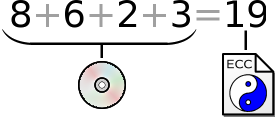
\includegraphics[height=28mm]{icons/ecc-example.png}
\end{minipage}
  &
\begin{minipage}{0.56\textwidth}
  For a given set of data (e.g. the numbers ``8 6 2 3'') additional
  error correction data (e.g. the sum ``19'') can be created so
  that a lost datum can be re-calculated from the remaining data.

  \smallskip
  
  The same principle is used in dvdisaster; the protected sequence
  of numbers is nothing else than the ISO image of an optical disc.
\end{minipage}
\end{tabular}

\bigskip

The concept of {\bf redundancy} can be explained as follows:

\begin{itemize}
\item  One ``error correction number'' is calculated for four input
  numbers. 1 of 4 (or 1/4) relates to a redundancy of 25\%.
\item  From one error correction number we can re-calculate exactly
  one missing number, or at most 25\% of data. The redundancy
  is equivalent to the maximum capacity of the error correction.
\item  Additional storage required for the error correction data is
  also determined by the redundancy (again, 25\% in the example).
\end{itemize}

dvdisaster uses the term of redundancy accordingly.
In addition please observe that

\begin{itemize}
\item  no data can be recovered when the data loss exceeds the
  redundancy (the equation in the example can not be solved for
  two or more unknowns).
\item the error correction data must be calculated at a
  point in time where all data is still present / readable.
\end{itemize}
  
The above shown example does not generalize into an error correction
scheme for recovering more than one missing data value. To do so a
more powerful equation system is needed which can be solved for more
than one missing value. dvdisaster uses a Reed-Solomon code which
does have such properties; however the required math is usually
not taught in school. Interested readers are therefore referred
to the respective books in coding theory. 

\newpage
\subsubsection{Using dvdisaster the right way}
\label{bigpicture-goodusage}

Let's demonstrate how Jane uses dvdisaster.

\bigskip

\begin{tabular}{rccl}
  10. Feb. 2009 &
  \begin{minipage}{16mm}\centerline{\goodcd}\end{minipage} &
  &
  \begin{minipage}{88mm}
    Jane creates a new CD with important data.
  \end{minipage}\\[8mm]

  &
  \begin{minipage}{16mm}\centerline{\goodcd}\end{minipage} &
  \begin{minipage}{16mm}\centerline{\eccfile}\end{minipage}  &
  \begin{minipage}{88mm}
    To protect the CD from data loss she creates
    \tlnk{howto-eccfile}{error correction data} with dvdisaster.
    She keeps both kinds of data for later usage.
  \end{minipage}\\[8mm]
  \hline

14. May 2010 &
  \begin{minipage}{16mm}\centerline{\goodcd}\end{minipage} &
  \begin{minipage}{16mm}\centerline{\eccfile}\end{minipage}  &
  \begin{minipage}{88mm}
    \vspace*{3mm}
    Jane knows that during daily use not all data of
    her CD might be accessed. So after a year has passed
    she \tlnk{howto-scan}{scans the CD for read errors} to make sure that
    it has not developed any defects in seldom used data regions.
    However after one year the CD is still perfectly readable.
    \vspace*{3mm}
  \end{minipage}\\[8mm]
  \hline

19. Aug 2012 &
  \begin{minipage}{16mm}\centerline{\badcd}\end{minipage} &
  \begin{minipage}{16mm}\centerline{\eccfile}\end{minipage}  &
  \begin{minipage}{88mm}
    \vspace*{3mm}
    Two more years have passed and Jane notices that
    some data on the CD is no longer readable.
    A \tlnk{howto-scan}{scan for read errors} confirms
    that the CD has become defective due to aging.
  \end{minipage}\\[8mm]

  \tlnk{howto-recover-read}{read} &
  \begin{minipage}{16mm}\centerline{\downarr}\end{minipage} &
  &
  \\[8mm]

  &
  \begin{minipage}{16mm}\centerline{\badimage}\end{minipage} &
  \begin{minipage}{16mm}\centerline{\eccfile}\end{minipage}  &
  \begin{minipage}{88mm}
    \vspace*{3mm}
    Jane uses dvdisaster
    to \tlnk{howto-recover-read}{read as much sectors as possible} from
      the defective CD into an ISO image.
  \end{minipage}\\[8mm]

  \tlnk{howto-recover-fix}{reconstruct} &
  \multicolumn{2}{c}{\begin{minipage}{32mm}\hspace*{5mm}\joinarr\end{minipage}} &
  \\[8mm]

  &
  \begin{minipage}{16mm}\centerline{\goodimage}\end{minipage} &
  \begin{minipage}{16mm}\centerline{\eccfile}\end{minipage}  &
  \begin{minipage}{88mm}
    By using the error correction data
    Jane \tlnk{howto-recover-fix}{recovers the missing parts} in
    the ISO image. 
  \end{minipage}\\[8mm]

  Write new CD&
  \begin{minipage}{16mm}\centerline{\downarr}\end{minipage} &
  &
  \\[8mm]

  &
  \begin{minipage}{16mm}\centerline{\goodcd}\end{minipage} &
  \begin{minipage}{16mm}\centerline{\eccfile}\end{minipage}  &
  \begin{minipage}{88mm}
    Jane writes a new CD from the recovered ISO image.
    She keeps the error correction data for the new CD
    as it may also become defective in the future.
  \end{minipage}\\[8mm]
\end{tabular}

\newpage
\subsubsection{Using dvdisaster the wrong way}
\label{bigpicture-badusage}

Joe bets on his media keeping their content without additional protection.

\bigskip

\begin{tabular}{rccl}
  10. Feb. 2009 &
  \begin{minipage}{16mm}\centerline{\goodcd}\end{minipage} &
  \begin{minipage}{16mm}\centerline{\goodcd}\end{minipage} &
  \begin{minipage}{88mm}
    Joe creates two CDs containing important data.
    But he does not make any provisions against data loss on those media.
  \end{minipage}\\[8mm]

  \hline
  
  \vspace*{3mm}
  14. May. 2010 &
  \begin{minipage}{16mm}
    \vspace*{3mm}
    \centerline{\goodcd}\end{minipage} &
  \begin{minipage}{16mm}
    \vspace*{3mm}
    \centerline{\goodcd}\end{minipage} &
  \begin{minipage}{88mm}
    Joe uses his CDs regularly. After one year they are
    still perfectly readable.
  \end{minipage}\\[4mm]

  \hline

  \vspace*{3mm}
  19. Aug. 2012 &
  \begin{minipage}{16mm}
    \vspace*{3mm}
    \centerline{\badcd}\end{minipage} &
  \begin{minipage}{16mm}
    \vspace*{3mm}
    \centerline{\goodcd}\end{minipage} &
  \begin{minipage}{88mm}
    After two more years Joe notices that some data
    on one CD is no longer readable.
  \end{minipage}\\[-1mm]

  \tlnk{howto-scan}{scan} &
  \begin{minipage}{16mm}\centerline{\downarr}\end{minipage} &
  \begin{minipage}{16mm}\centerline{\downarr}\end{minipage} &
  \\[-1mm]

  20. Aug. 2012 &
  \begin{minipage}{16mm}
    \centerline{\badcd}\end{minipage} &
  \begin{minipage}{16mm}
    \centerline{\badcd}\end{minipage} &
  \begin{minipage}{88mm}
    Joe downloads dvdisaster and performs
    a \tlnk{howto-scan}{read error scan}.
    He finds out that the CD contains 25000 unreadable sectors.
    A scan of the second CD reveals that it has developed 1500
    unreadable sectors gone unnoticed so far. 
  \end{minipage}\\[-2mm]

  \tlnk{howto-recover}{reading} &
  \begin{minipage}{16mm}\centerline{\downarr}\end{minipage} &
  \begin{minipage}{16mm}\centerline{\downarr}\end{minipage} &
  \\[5mm]

  21. Aug. 2012 &
  \begin{minipage}{16mm}
    \centerline{\badimage}\end{minipage} &
  \begin{minipage}{16mm}
    \centerline{\badimage}\end{minipage} &
  \begin{minipage}{88mm}
    Joe uses dvdisaster to read as much sectors as
    possible from the defective media. But since he
    does not have error correction data there is no way
    of recalculating the unreadable sectors.
  \end{minipage}\\[6mm]

  \begin{minipage}{20mm}
    many reading attempts
  \end{minipage}
    &
  \begin{minipage}{16mm}\centerline{\downarr}\end{minipage} &
  \begin{minipage}{16mm}\centerline{\downarr}\end{minipage} &
  \\[-10mm]

  05. Sep. 2012 &
  \begin{minipage}{16mm}
    \centerline{\badimage}\end{minipage} &
  \begin{minipage}{16mm}
    \centerline{\goodimage}\end{minipage} &
  \begin{minipage}{88mm}
    Joe takes advantage of dvdisaster's feature to complete images
    through multiple reading passes. He moves the defective images
    to several computers to perform reading attempts with
    different drives. After two weeks of trying at least all
    missing sectors from the second CD have been read. However
    on the first CD still 21000 sectors remain unreadable by any
    drive he tried.
  \end{minipage}\\[-4mm]

  \begin{minipage}{25mm}
    only one CD recovered
  \end{minipage}
    &
  \begin{minipage}{16mm}\centerline{\downarr}\end{minipage} &
  \begin{minipage}{16mm}\centerline{\downarr}\end{minipage} &
  \\[-2mm]

  06. Sep. 2012 &
  \begin{minipage}{16mm}
    \centerline{\badcd}\end{minipage} &
  \begin{minipage}{16mm}
    \centerline{\goodcd}\end{minipage} &
  \begin{minipage}{88mm}
    Joe dismisses the first CD as unrecoverable and
    considers himself lucky to have a complete image
    from the second CD again. However if he had created
    error correction data in time, he'd probably\footnotemark
    saved two weeks of reading attempts and recovered
    the contents from both CDs.
  \end{minipage}\\[8mm]
\end{tabular}

\footnotetext{The
  error correction assumes a typical aging process. If the CD
  gets severely damaged it becomes unrecoverable even with
  error correction data. Do not rely on dvdisaster alone
  for protecting important data; instead employ additional
  measures like creating additional copies on different types of media.}

\newpage

\subsection{Scanning media for errors}
\label{howto-scan}

\begin{tabular}{lll}
  \multicolumn{2}{l}{\bf Task} &
  The medium is scanned for unreadable sectors. \\[10mm]

  \multicolumn{2}{l}{\bf Required:} & \\[3mm]

  \begin{minipage}{15mm}
    \goodcd
  \end{minipage} &

  \begin{minipage}{15mm}
    \badcd
  \end{minipage} &

  A medium in any state (good or containing read errors) \\[10mm]

  \begin{minipage}{15mm}
    \eccfile
  \end{minipage} &
  &
  \begin{minipage}{110mm}
  If error correction data is available additional tests are
  carried out. However scanning will also work without error correction
  data.
  \end{minipage}
  \\[13mm]

  \multicolumn{2}{l}{\bf What to do:} &
  \tlnk{howto-scan-basic-settings}{1. Configure basic settings} \\[2mm]

  & &
  \tlnk{howto-scan-walkthrough}{2. Scan the medium} \\[2mm]

  & &
  \tlnk{howto-scan-interpret}{3. Interpret the results} \\[10mm]


  \multicolumn{2}{l}{\bf Related functions:} &
  \tlnk{howto-recover-read}{Reading of damaged media} and \\[2mm]

  & &
  \tlnk{howto-recover-fix}{recovering images} \\[2mm]
\end{tabular}

\vspace{10mm}

\subsubsection{Basic settings}
\label{howto-scan-basic-settings}

\begin{figure}[h]
\centerline{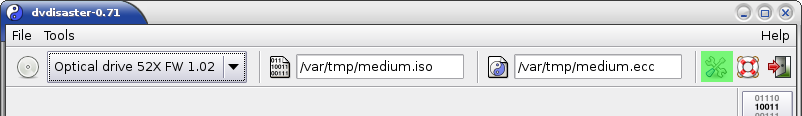
\includegraphics[width=\textwidth]{screenshots/global-prefs-invoke.png}}
\caption{Opening the configuration dialog.}  
\label{howto-scan-open-preferences}
\end{figure}

The relevant tabs are described on the next pages. They are
found in the configuration dialog.
Open the dialog by selecting the symbol marked green in the
screen shot ( \begin{minipage}{8mm}
\includegraphics{icons/prefs-icon.png}\end{minipage}, see figure \ref{howto-scan-open-preferences}).
The symbol may look different due to the symbol theme you are using.

\newpage

\begin{figure}[h]
\centerline{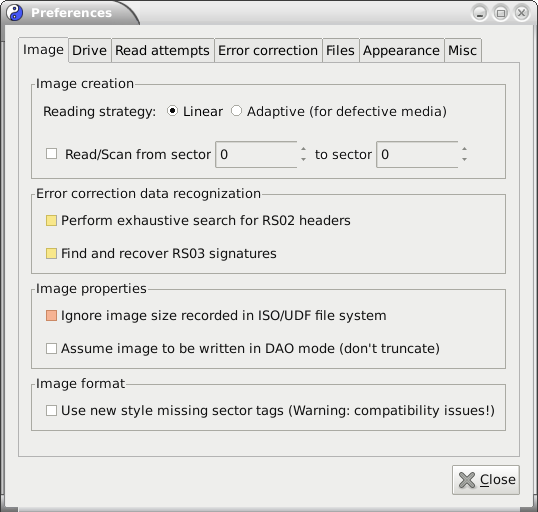
\includegraphics[width=0.9\textwidth]{screenshots/scan-prefs-image.png}}
\caption{The ``Image'' tab.}  
\label{howto-scan-prefs-image}
\end{figure}

\paragraph{Error correction data recognization.} If you
are sure that your medium contains embedded RS02 or RS03 error
correction data, activate the respective items (marked yellow).
Using the error correction (ecc) data will improve scanning results,
but searching for non existing ecc data will cost several minutes.

\paragraph{Image properties.} Selecting the proper
method for determining the image size is important.
Make sure that ``Ignore image size recorded in ISO/UDF file system''
(marked red) is switched off.
This option should only be used
in \tlnk{howto-eccfile-advanced-settings-image}{special cases during image recovery}.

\smallskip

Adjust the remaining settings as shown in the screen shot.

\newpage

\begin{figure}[h]
\centerline{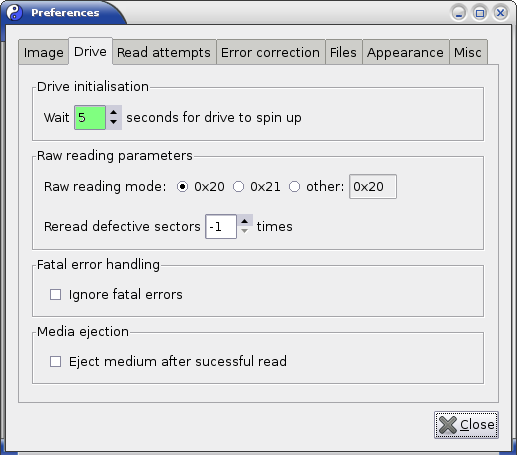
\includegraphics[width=0.9\textwidth]{screenshots/scan-prefs-drive.png}}
\caption{The ``Drive'' tab.}  
\label{howto-scan-prefs-drive}
\end{figure}

\paragraph{Drive initialization.} Reading data
from the drive while it is spinning up can generate spurious error
reports. Adjust the spin up time for your drive (typically 5-10 seconds)
in the field marked green to make dvdisaster wait for the appropriate time.

\smallskip

Leave the other settings at the values shown; you
can \tlnk{howto-scan-advanced-settings}{optimize} them later.

\newpage

\begin{figure}[h]
\centerline{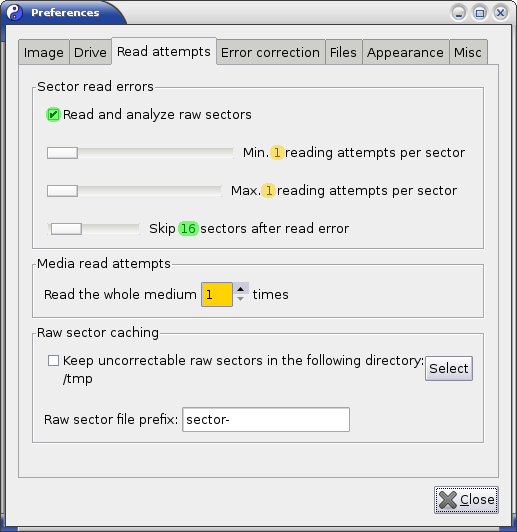
\includegraphics[width=0.9\textwidth]{screenshots/scan-prefs-read-attempts.png}}
\caption{The ``Read attempts'' tab.}  
\label{howto-scan-prefs-read-attempts}
\end{figure}

\paragraph{Sector read errors.} The option ``Read and analyse raw sectors''
(first green marking) uses C2 analysis and possibly more raw data
reported by the drive for a better assessment of CD media quality.
This setting does nothing for DVD and BD media, but it is safe to
remain activated unless it causes problems with your drive reading CDs.

Adjust the reading attempts settings as shown here. Using larger
values causes unnecessary reading activity but will not improve the scan.
After a read error no less than 16 sectors should be skipped (second
green marking); when scanning badly damaged media this setting can
be \tlnk{howto-scan-advanced-settings-read-attempts}{optimized using larger values}.

\paragraph{Media read attempts.} Performing multiple read attempts
is not recommended during a scan; set the number of retries to 1
in the three places marked in orange. Collecting raw sectors should
also be off during the scan.

\newpage

\begin{figure}[h]
\centerline{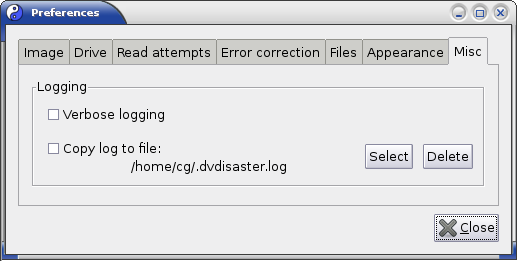
\includegraphics[width=0.9\textwidth]{screenshots/general-prefs-misc.png}}
\caption{The ``Misc'' tab.}  
\label{howto-scan-prefs-misc}
\end{figure}

\paragraph{The ``Misc Tab''.} Currently
this tab only has functions for creating log files.
This is helpful for \tlnk{reporting-defects}{reporting defects} but
should be left off during normal operation.

\paragraph{Not used tabs.} The ``Error correction'' and ``Files'' tabs
have no influence on scanning media. The ``Appearance'' tab
allows you to adapt the output colors to your taste, but these have
no further effects on the scanning process. 

\newpage
\subsubsection{Scanning for errors - Walkthrough}
\label{howto-scan-walkthrough}

Please make sure that dvdisaster has been configured as
described in the \tlnk{howto-scan-basic-settings}{basic settings} section
as some settings might negatively affect the scanning results.
Then perform the following steps: 

\bigskip

\begin{tabular}{cl}
  \begin{minipage}{50mm}
    \centerline{\slotin}
  \end{minipage}
  &
  \begin{minipage}{104mm}
  {\bf Insert the medium you want to scan into a drive} which
  is directly connected to your computer. You can not use network
  drives, software drives and drives inside virtual machines.
  \end{minipage}\\

  \begin{minipage}{50mm}
    \centerline{\downarr}
  \end{minipage}
  & \\

  \begin{minipage}{50mm}
    \centerline{\filemanager}
  \end{minipage}
  &
  \begin{minipage}{104mm}
    {\bf Close any windows} which may be opened by your
    operating system for viewing or performing the medium contents.
    Wait until the drive has recognized the medium and the medium
    has spun down. 
  \end{minipage}\\

  \begin{minipage}{50mm}
    \centerline{\downarr}
  \end{minipage}
  & \\[6mm]

  \begin{minipage}{50mm}
    \centerline{\selectdrive}
  \end{minipage}
  &
  \begin{minipage}{104mm}
    {\bf Select the drive containing the medium} in dvdisasters
    drop down menu. 
  \end{minipage}\\[4mm]

  \begin{minipage}{50mm}
    \centerline{\downarr}
  \end{minipage}
  & \\

  \begin{minipage}{50mm}
    \centerline{\selectecc}
  \end{minipage}
  &
  \begin{minipage}{104mm}
    {\bf Select the error correction file for this medium} if you
    have one available. Ecc data from RS02 or RS03 augmented media
    is used automatically.
  \end{minipage}\\

  \begin{minipage}{50mm}
    \centerline{\downarr}
  \end{minipage}
  & \\[6mm]

  \begin{minipage}{50mm}
    \centerline{\scanicon}
  \end{minipage}
  &
  \begin{minipage}{104mm}
    Start the scan by {\bf clicking the "Scan" button.}
  \end{minipage}\\[6mm]

  \begin{minipage}{50mm}
    \centerline{\downarr}
  \end{minipage}
  & \\[6mm]

  \begin{minipage}{50mm}
    \centerline{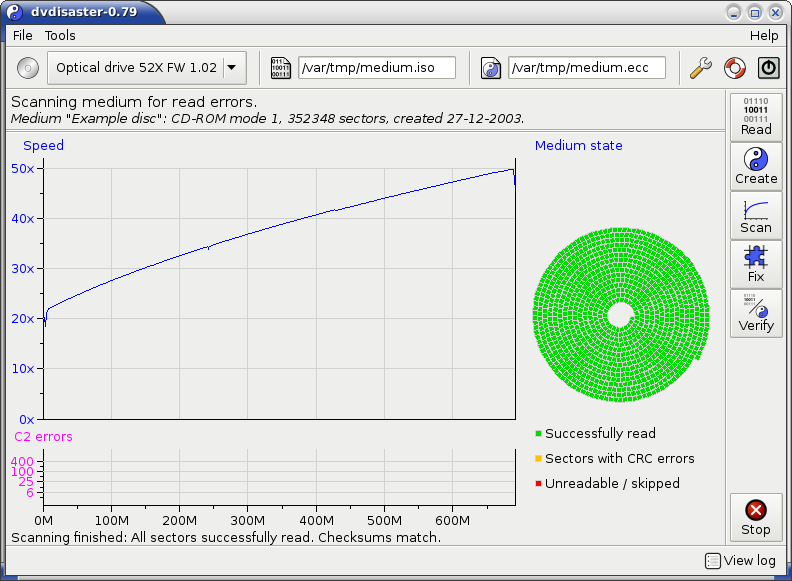
\includegraphics[width=40mm]{screenshots/good-cd-scan.png}}
  \end{minipage}
  &
  \begin{minipage}{104mm}
    {\bf Watch the scanning progress.} Do not perform any other
    actions on your computer while the scan is running.
    Opening or working with other programs as well as moving
    other windows around might affect the scanning results. 
  \end{minipage}\\
\end{tabular}

\newpage
\subsubsection{Interpreting the results}
\label{howto-scan-interpret}

\begin{figure}[h]
\centerline{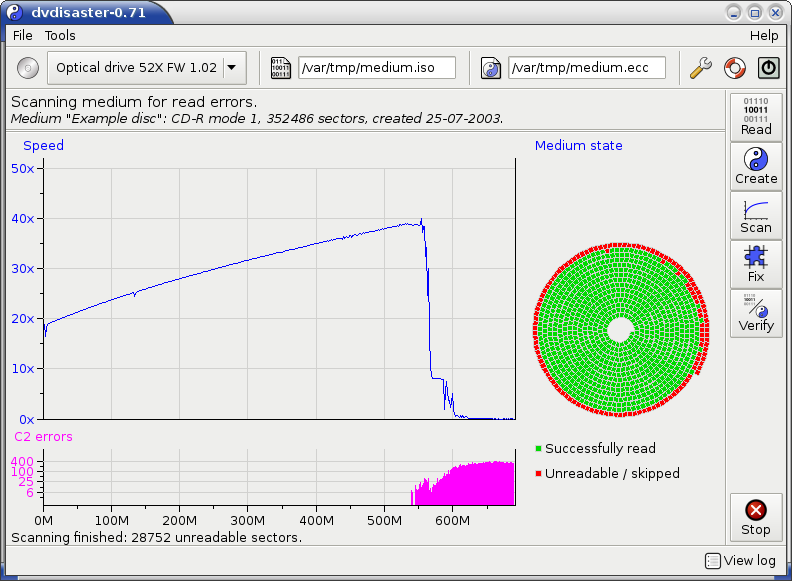
\includegraphics[width=0.97\textwidth]{screenshots/defective-cd-scan.png}}
\caption{Scanning the medium.}  
\label{howto-scan-general-results}
\end{figure}

\vspace*{-5mm}

\paragraph{Overview.} dvdisaster provides several information
about the scanning results (see fig. \ref{howto-scan-general-results}): 

\begin{itemize}
  \item The spiral under {\bf ``Medium State''} (to the right).

    The spiral provides information about the medium readability.
    The medium is fully readable when all segments of the spiral
    are colored green. Yellow or red blocks mark places where data
    could not be correctly read from the medium. The total number
    of unreadable sectors is printed in the ``Scanning finished:''
    message at the window bottom.

  \item {\bf ``Speed''} - The reading speed curve (upper left).

    The reading speed is not an absolute gauge of the medium
    health, but it is usable as a rule of thumb: The more
    regular the curve, the better the medium. You will
    find examples of good and bad reading speed curves on the following pages.

  \item {\bf ``C2 errors''} - A medium state gauge provided by the drive (down left).

    This kind of analysis is \tlnk{qa-quality-scans}{currently only available for CD media}.
    CD drives have a built-in error correction
    which can eliminate small data losses caused by minor
    defects on the medium. The number of C2 errors is a
    measurement of how often the drive needed to employ its
    internal error correction during the read - this value
    should be zero on good media.
\end{itemize}

\newpage
\begin{figure}[h]
\centerline{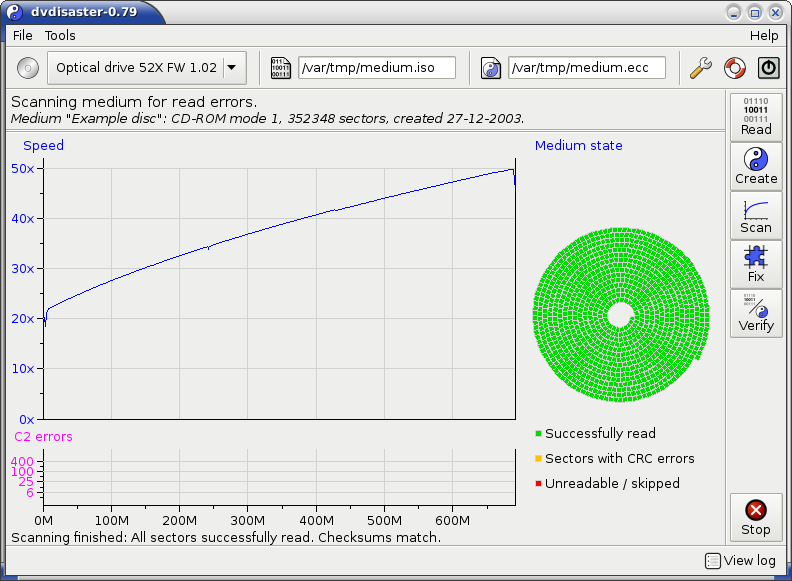
\includegraphics[width=\textwidth]{screenshots/good-cd-scan.png}}
\caption{Good CD.}  
\label{howto-scan-good-cd}
\end{figure}

{\bf Example of a good medium:} This screen shot shows
a perfect CD: All blocks under ``Medium state'' are green, no C2
errors have been reported and the reading curve runs smoothly.
A rising reading speed is normal for most media (see the next screen
shot for a counter example). The small spikes at the beginning and
at the end of the curve are normal; minor glitches like the one shown
at 250M are also harmless.

\newpage
\begin{figure}[h]
\centerline{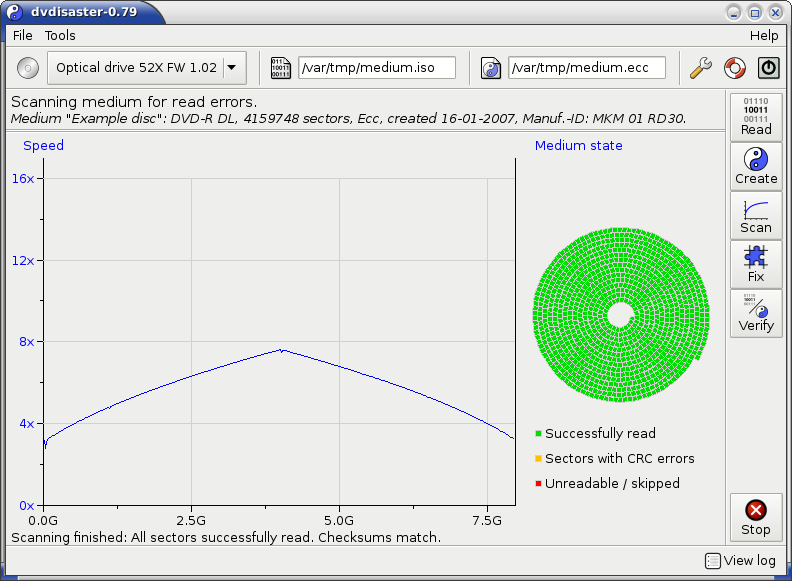
\includegraphics[width=\textwidth]{screenshots/good-dvd9-scan.png}}
\caption{Good two-layered DVD.}  
\label{howto-scan-good-two-layered-dvd}
\end{figure}

{\bf Sometimes the reading curve won't rise steadily:} Multi-layered
media might yield reading curves which are rising and dropping
in a symmetric pattern. Not shown but also possible are flat
curves without any change in reading speed (most typically seen
with DVD-RAM).

\newpage
\begin{figure}[h]
\centerline{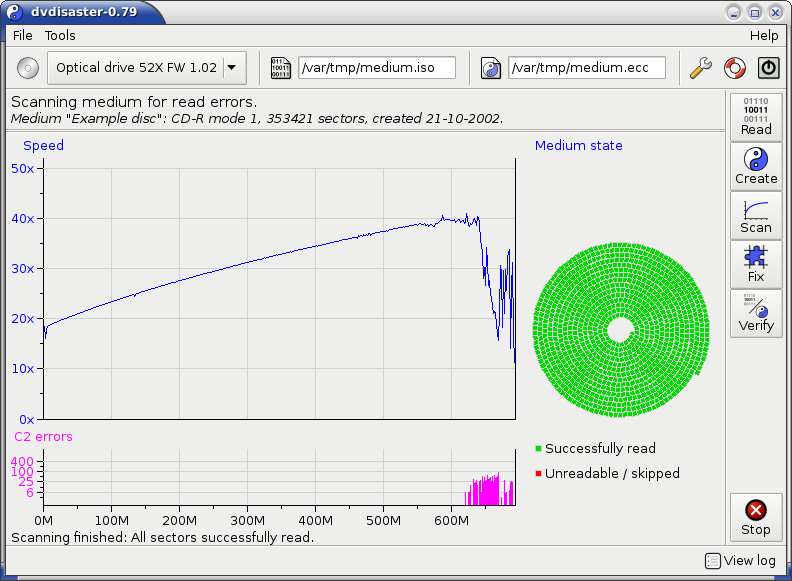
\includegraphics[width=\textwidth]{screenshots/weak-cd-scan.png}}
\caption{Weak CD.}  
\label{howto-scan-weak-cd}
\end{figure}

{\bf An example of a weak medium.} This medium is still
readable as indicated by the green spiral shown under ``Medium state''.
However there are clear signs of serious trouble ahead: The drive must
slow down significantly towards the end of the medium in order to read
from it. Note the steep fall of reading speed after the 600M mark.
This comes along with C2 error rates rising to the 100 mark; this is
another warning that the medium is decaying in the outer region.
If you have not created \tlnk{howto-ecc}{error correction data} this is probably the
last opportunity to do so as the medium will develop the first
read errors soon.

\newpage
\begin{figure}[h]
\centerline{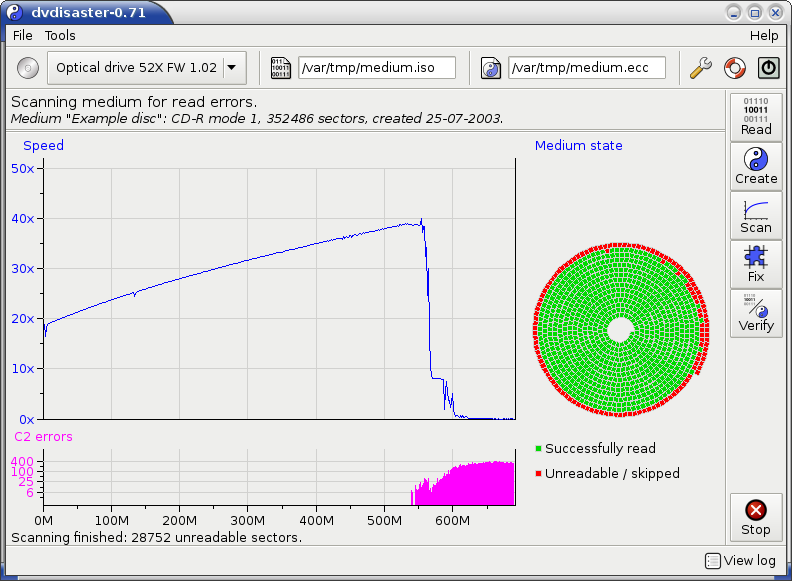
\includegraphics[width=\textwidth]{screenshots/defective-cd-scan.png}}
\caption{Defective CD.}  
\label{howto-scan-defective-cd}
\end{figure}

{\bf Example of a defective CD.} \label{howto-interpret-defective-cd}
The red sectors in the spiral
visualize large unreadable sections in the outer region of the medium.
At the bottom of the window you will find the information that the
medium contains 28752 unreadable sectors. This sums up to about
8.2\% defective sectors (of 352486 sectors total) and is well within
the \tlnk{howto-recover}{recovery} bounds
by \tlnk{howto-ecc}{error correction (ecc) data} made with default
settings - if you have made the ecc data in time! Otherwise the
contents of the red sectors are lost since ecc data cannot be
created from already defective media.

\newpage
\begin{figure}[h]
\centerline{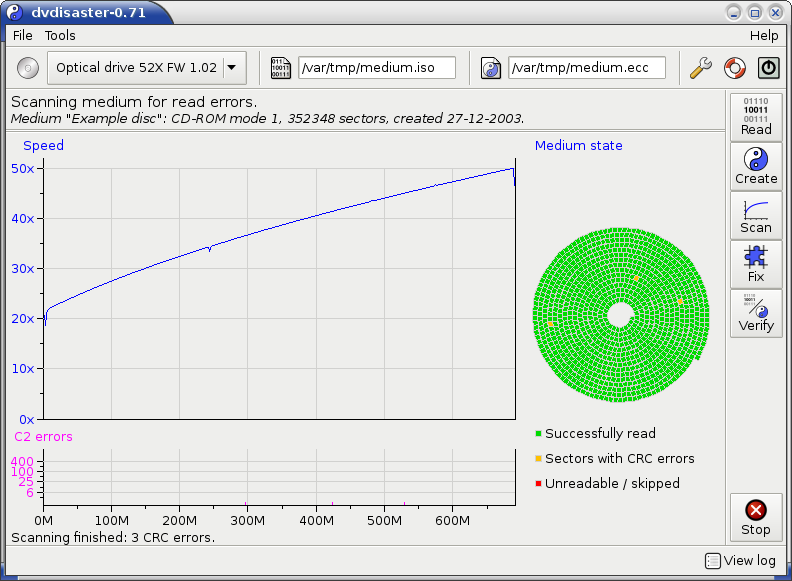
\includegraphics[width=\textwidth]{screenshots/crc-cd-scan.png}}
\caption{Checksum errors.}  
\label{howto-scan-checksum-errors}
\end{figure}

{\bf Checksum errors.} Yellow spots in the spiral depict places
where the medium was fully readable, but the data read did not
match checksums in the error correction data. There are two main causes:

\begin{itemize}
\item The image has been manipulated after the creation of
  error correction data and before writing it to the medium.
  This can happen when the image is mounted with
  write access after ecc data has been created. Typical signs are
  CRC errors in sector 64 and in sectors 200 to 400 as the system
  updates the file access times there. Performing a data recovery
  using dvdisaster is typically harmless in this situation.

  \medskip

  However if you have modified files in the image after
  creating the ecc data, the error correction data will be both
  worthless and dangerous. Applying a recovery to the medium will
  restore the image state at the time the ecc data has been created,
  and this will obviously not represent the most recent contents of
  the medium.

\item There are technical problems with the computer system,
  especially in mass storage communication. Perform the scan again
  and observe the CRC error locations. If CRC errors disappear
  or surface at different locations your system might have
  defective RAM, bad drive cabling/controllers or incorrect clock speeds.
\end{itemize}

\newpage
\subsubsection{Advanced settings}
\label{howto-scan-advanced-settings}

\begin{figure}[h]
\centerline{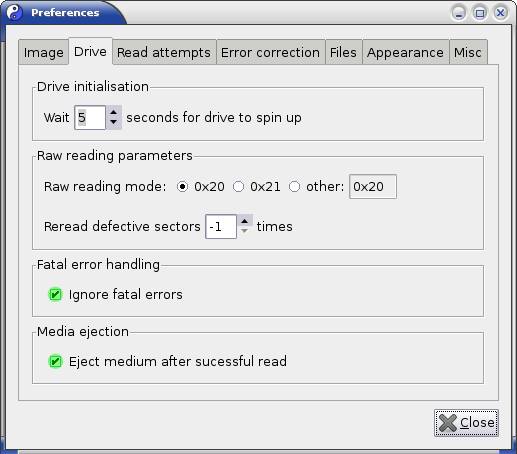
\includegraphics[width=0.9\textwidth]{screenshots/scan-prefs-drive-adv.png}}
\caption{Advanced settings in the ``Drive'' tab.}  
\label{howto-scan-prefs-drive-adv}
\end{figure}

{\bf Fatal error handling.} dvdisaster will normally abort the scan
when the drive reports a fatal internal error like mechanical problems.
The intention is to avoid damaging the drive. However some drives
will erroneously report such problems when they get confused by
damaged media. If you have such a drive you can use this option
to force the scan to continue.

\bigskip

{\bf Media ejection.} dvdisaster tries to eject the medium after
a successful scan if this option is activated. However ejecting
the medium might be prohibited by the operating system so this
is not guaranteed to work. For example if upon media insertion
a window is opened for performing the contents it may not be
possible to automatically eject the medium.

\newpage
\begin{figure}[h]
\centerline{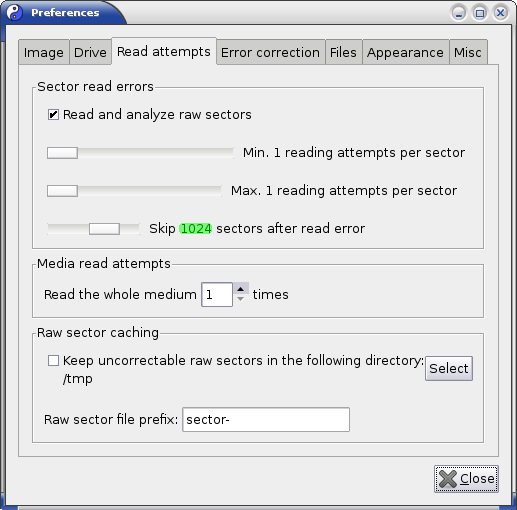
\includegraphics[width=0.9\textwidth]{screenshots/scan-prefs-read-attempts-adv.png}}
\caption{Advanced settings in the ``Read attempts'' tab.}  
\label{howto-scan-prefs-read-attempts-adv}
\end{figure}

{\bf Sector read errors.} \label{howto-scan-advanced-settings-read-attempts} Attempts
for reading defective sectors
cost a lot of time. Since it is likely to encounter another defective
sector after hitting a read error, skipping a few sectors after a
read error saves time and reduces wear on the drive. If you only want
a quick overview of a damaged medium setting this value to 1024 might help.
But keep in mind that all skipped sectors are counted as being defective
so the number of reported errors becomes higher and less accurate.

\newpage
\subsection{Selecting the right type of ecc data}
\label{howto-ecc}

Error correction data can either be created in form of
a separate error correction file or it can be placed directly
onto the medium.

\smallskip

Answering the following questions can quickly guide you to the right
ecc data format:

\begin{itemize}
\item {\em Do you need error correction data for a medium which has already been written?}

  In that case, you need to \tlnk{howto-eccfile}{create an error
    correction file} because an already existing medium can not be
  augmented with error correction data. 

\item {\em Are you planning to write the medium right now?}

  If the medium is full or nearly full (less than 20\% free),
  not enough space might be available for storing the error
  correction data. It is strongly recommended to \tlnk{howto-eccfile}{create an
  error correction file} in that case. Otherwise, you can put
  the \tlnk{howto-augment}{error correction data directly onto the medium}.
  To do so you must create an ISO image first and then augment it with
  error correction data before you write it to the medium. 
\end{itemize}

\paragraph{More information on keeping error correction data.}\quad

dvdisaster helps protecting your media from data loss by
forehanded\footnote{ Let's repeat again for clarity: Error correction data
  must be created before the medium becomes defective. It is not possible
  to create error correction data from defective media; in that case
  unreadable sectors can not be recovered.} creation of error correction
data. Error correction data must be treated like normal backup data,
e.g. you need to keep it available during the whole lifetime of the
respective medium.

\smallskip

The easiest way is storing the error correction data on the medium
you want to protect. But this is only possible if the medium has not
yet been written: To employ this method you need to create an ISO image
first, then augment this image with error correction data, and finally
write the augmented image to the medium.

\smallskip

If the medium has already been written, or insufficient space is left
for augmenting the image, you still can create error correction data
in form of a free-standing error correction file. This file must then
be stored somewhere else, e.g. you need to take additional provisions
to \tlnk{howto-eccfile-archival}{archive your error correction files}.

\smallskip

More information about the pro and con of these methods can be found
in the \tlnk{background-methods}{background information} section. 

\newpage

\subsection{Creating ecc data as a separate file}
\label{howto-eccfile}

\begin{tabular}{ll}
  {\bf Task} & An error correction file is created for an optical medium. \\

  &
  \begin{minipage}{132mm}

    \bigskip

    Note: This page describes how error correction data is created
    and placed into a separate file. There is also a method for
    placing the error correction data \tlnk{howto-augment}{directly onto the medium}.

    \smallskip
    
    \tlnk{howto-ecc}{Would you like help on deciding between these two methods?}
    \end{minipage}\\[15mm]
    
  {\bf Required:} & \\[3mm]

  \begin{minipage}{15mm}
    \goodcd
  \end{minipage} &
  \begin{minipage}{132mm}
    A good, error free\footnotemark medium,
  \end{minipage} \\

  & or \\

  \begin{minipage}{15mm}
    \goodimage
  \end{minipage} &
  \begin{minipage}{132mm}
    \addtocounter{footnote}{-1}
    an already existing and complete\footnotemark ISO
    image of the medium (e.g. the image used for
    writing the medium). 
  \end{minipage} \\[10mm]

  {\bf What to do:} &
  \tlnk{howto-eccfile-basic-settings}{1. Configure basic settings} \\[2mm]

  &
  \tlnk{howto-eccfile-create}{2. Create the error correction file} \\[2mm]

  &
  \tlnk{howto-eccfile-archival}{3. Archive the error correction file}
\end{tabular}

\footnotetext{Error correction data must be
      created before any data loss occurs: It is not possible
      to create error correction files from an already defective
      medium.}

\vspace{10mm}

\subsubsection{Basic settings for reading the image from the medium}
\label{howto-eccfile-basic-settings}
\label{howto-eccfile-basic-settings-reading}

\begin{figure}[h]
\centerline{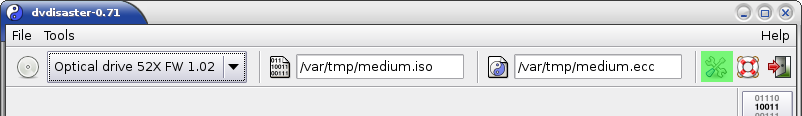
\includegraphics[width=\textwidth]{screenshots/global-prefs-invoke.png}}
\caption{Opening the configuration dialog.}  
\label{howto-eccfile-open-preferences-eccfile}
\end{figure}

The relevant tabs are described on the next pages. They are
found in the configuration dialog.
Open the dialog by selecting the symbol marked green in the
screen shot ( \begin{minipage}{8mm}\includegraphics{icons/prefs-icon.png}\end{minipage}, see figure \ref{howto-eccfile-open-preferences-eccfile}).
The symbol may look different due to the symbol theme you are using.

\bigskip

\begin{tabular}{cl}
  \begin{minipage}{20mm}
    \centerline{\goodimage}
  \end{minipage} &
  \begin{minipage}{133mm}
      If you already have an ISO image available you can skip the next
      three tabs and proceed with
      the \tlnk{howto-eccfile-basic-settings-ecc}{error correction settings}.
      But make sure that you really have an ISO type image; other formats
      like ``.nrg'' do not produce usable error correction data.
    \end{minipage}\\
 \end{tabular}
    
\newpage

\begin{figure}[h]
\centerline{\includegraphics[width=0.9\textwidth]{screenshots/eccfile-prefs-image.png}}
\caption{The ``Image'' tab.}  
\label{howto-eccfile-prefs-image}
\end{figure}

\paragraph{Reading strategy.} Make sure that the linear reading strategy is selected
(marked green).

\bigskip

All other options should be turned off; especially those marked green as they
might have adverse effects on the image reading process. 

\newpage

\begin{figure}[h]
\centerline{\includegraphics[width=0.9\textwidth]{screenshots/eccfile-prefs-drive.png}}
\caption{The ``Drive'' tab.}  
\label{howto-eccfile-prefs-drive}
\end{figure}

\paragraph{Drive initialization.} Reading data from the drive while it is spinning
up can generate spurious error reports. Adjust the spin up time for your
drive (typically 5-10 seconds) in the field marked green to make dvdisaster
wait for the appropriate time.

\bigskip

Leave the other settings at the shown values.

\newpage

\begin{figure}[h]
\centerline{\includegraphics[width=0.9\textwidth]{screenshots/eccfile-prefs-read-attempts.png}}
\caption{The ``Read attempts'' tab.}  
\label{howto-eccfile-prefs-read-attempts}
\end{figure}

\paragraph{Sector read errors.} The option ``Read and analyze raw sectors'' (marked green)
uses additional information provided by the drive to check the integrity of read data.
This is recommended as we are interested in creating error correction data
from a properly read image.

\medskip

On the other hand since error correction data can only be created from fully
readable media we do not need multiple reading attempts and caching of
raw sectors as shown in the screen shot. 

\newpage
\subsubsection{Basic settings for the error correction data}
\label{howto-eccfile-basic-settings-ecc}

\begin{figure}[h]
\centerline{\includegraphics[width=0.9\textwidth]{screenshots/eccfile-prefs-ecc-file3.png}}
\caption{The ``Error correction'' tab for the RS03 codec.}  
\label{howto-eccfile-prefs-ecc-file3}
\end{figure}

Error correction files can be created using either the RS03 or the RS01 method
(see this \tlnk{background-methods}{comparison} for details).
It is recommended to use RS03 as it contains all features present in RS01,
but encodes much faster due to certain optimizations.

\paragraph{Settings for encoding with the RS03 method.} First select the entry
``Multithreaded RS codec (RS03)'' in the drop down menu (marked green).
After this selection the contents of the tab will display the choices given
for the RS03 method. 

\paragraph{Error correction storage.} Select ``File'' (also marked green).
This option causes error correction data to be stored in a separate file
and will also make the redundancy choice available which is located below.

\paragraph{Redundancy for new error correction files.} Select the redundancy
which suits your needs. The redundancy will determine the maximum error
correction capability: An error correction file with x\% redundancy can
correct up to x\% of read errors under optimal circumstances.
Since the best case is usually not encountered you should add some safety
margin to the redundancy by picking one of the following choices (see yellow markings):

\begin{itemize}
\item The ``normal'' and ``high'' presets provide a redundancy of 14.3\% and 33.5\%
  respectively.
\item You can freely choose the redundancy by activating the ``other'' item
  and dragging the slider.
\item By activating the ``Use at most'' button you can specify the error
  correction file size in MiB. dvdisaster will choose a suitable redundancy
  so that the error correction file will be close to but not larger than the
  specified size.
\end{itemize}
  
The redundancy will also determine the size of the error correction file;
using x\% redundancy will create an error correction file of about x\% the
size of the image. Using redundancies lower than the ``normal'' setting (14.3\%)
is not recommended as the error correction might be overloaded too quickly.

\paragraph{Multithreading.} The RS03 encoder can distribute its workload
onto multiple processor cores by using multithreading. On machines with
up to four cores, set the number of threads equal to the number of
cores (e.g. use 4 threads on a 4 core machine). On machines with more
than 4 cores, use one thread less than the number of available cores;
e.g. use 7 threads on an 8 core machine - this leaves one core free
for housekeeping tasks).

\smallskip

Leave the other settings as shown in the screenshot; you can
\tlnk{howto-eccfile-advanced-settings-ecc}{optimize} them later.

\newpage

\begin{figure}[h]
\centerline{\includegraphics[width=0.9\textwidth]{screenshots/eccfile-prefs-ecc-file1.png}}
\caption{The ``Error correction'' tab for the old RS01 codec.}  
\label{howto-eccfile-prefs-ecc-file1}
\end{figure}

\paragraph{Settings for encoding with the RS01 method.} If you want to
use the old RS01 method, choose ``Error correction file (RS01)'' in
the ``Storage method'' drop down menu (green marking; see
fig. \ref{howto-eccfile-prefs-ecc-file1}).

\smallskip

Then select a redundancy setting which suits your needs; see the
explanations on redundancy for the RS03 method above for more information.
For RS01, the ``normal'' and ``high'' settings are somehow optimized for
speed, but still much slower than their RS03 counterparts. 

\newpage

\begin{figure}
\centerline{\includegraphics[width=0.9\textwidth]{screenshots/create-prefs-file.png}}
\caption{The ``Files'' tab.}  
\label{howto-eccfile-prefs-file}
\end{figure}

\paragraph{The ``Files'' tab.} In this tab, only
activate the option for confirming file overwriting.
Leave the other options off for the moment; suggestions for
further \tlnk{howto-eccfile-advanced-settings}{optimization} follow later. 

\bigskip

\paragraph{Not used tabs.} The ``Misc'' tab currently has only functions
for creating log files. This is helpful
for \tlnk{reporting-defects}{reporting defects} but
should be left off during normal operation. The ``Appearance'' tab allows
you to adapt the output colors to your taste, but these have no further
effects on the error correction data creation.

\newpage
\subsubsection{Creating the error correction file}
\label{howto-eccfile-create}

\begin{tabular}{cccl}
  \begin{minipage}{15mm}
    \goodcd
  \end{minipage}
  &
  \begin{minipage}{10mm}
    \rightarr
  \end{minipage}
  &
  \begin{minipage}{15mm}
    \goodimage
  \end{minipage}
  &
  \begin{minipage}{105mm}
    The error correction file can only be created from an ISO image
    on hard disk, not directly from the medium. If you have the
    ISO image already/still available from making the medium,
    turn over to the next page. Otherwise, follow these instructions
    for extracting the ISO image from the medium.
  \end{minipage}
  \\
\end{tabular}

\bigskip

\hrulefill

\bigskip

\begin{tabular}{cl}
  \begin{minipage}{50mm}
    \centerline{\slotin}
  \end{minipage}
  &
  \begin{minipage}{104mm}
  {\bf Insert the medium you want to read into a drive} which
  is directly connected to your computer. You can not use network
  drives, software drives and drives inside virtual machines.
  \end{minipage}\\

  \begin{minipage}{50mm}
    \centerline{\downarr}
  \end{minipage}
  & \\

  \begin{minipage}{50mm}
    \centerline{\filemanager}
  \end{minipage}
  &
  \begin{minipage}{104mm}
    {\bf Close any windows} which may be opened by your
    operating system for viewing or performing the medium contents.
    Wait until the drive has recognized the medium and the medium
    has spun down. 
  \end{minipage}\\

  \begin{minipage}{50mm}
    \centerline{\downarr}
  \end{minipage}
  & \\[6mm]

  \begin{minipage}{50mm}
    \centerline{\selectdrive}
  \end{minipage}
  &
  \begin{minipage}{104mm}
    {\bf Select the drive containing the medium} in dvdisasters
    drop down menu. 
  \end{minipage}\\[4mm]

  \begin{minipage}{50mm}
    \centerline{\downarr}
  \end{minipage}
  & \\

  \begin{minipage}{50mm}
    \centerline{\selectimage}
  \end{minipage}
  &
  \begin{minipage}{104mm}
    {\bf Select a directory and file name} for
    storing the ISO image.
  \end{minipage}\\[4mm]

  \begin{minipage}{50mm}
    \centerline{\downarr}
  \end{minipage}
  & \\

  \begin{minipage}{50mm}
    \centerline{\readicon}
  \end{minipage}
  &
  \begin{minipage}{104mm}
    {\bf Create the ISO image} by clicking the "Read" button.
  \end{minipage}\\[6mm]

  \begin{minipage}{50mm}
    \centerline{\downarr}
  \end{minipage}
  & \\[6mm]

  \begin{minipage}{50mm}
    \centerline{\includegraphics[width=40mm]{screenshots/good-cd-scan.png}}
  \end{minipage}
  &
  \begin{minipage}{104mm}
    {\bf Watch the reading progress.}
    Wait until the medium has been completely read.
    If the medium turns out to contain defective sectors
    it will not be possible to create error correction data. 
  \end{minipage}\\
\end{tabular}

\bigskip
  
Now continue with the next page to create an error correction file
from the ISO image.

\newpage
\label{howto-eccfile-create-ecc}

\begin{tabular}{cccl}
  \begin{minipage}{15mm}
    \goodimage
  \end{minipage}
  &
  \begin{minipage}{10mm}
    \rightarr
  \end{minipage}
  &
  \begin{minipage}{15mm}
    \eccfile
  \end{minipage}
  &
  \begin{minipage}{105mm}
    Now that we have an ISO image of the medium, we can create the
    error correction file from it. It you do not have the ISO image yet,
    please follow the instructions on the previous page for
    extracting it from the medium.
  \end{minipage}
  \\
\end{tabular}

\bigskip

\hrulefill

\bigskip

\begin{tabular}{cl}
  \begin{minipage}{50mm}
    \centerline{\selectimage}
  \end{minipage}
  &
  \begin{minipage}{104mm}
    {\bf Select the directory and name of the ISO image} for which you want 
    to create the error correction data. It is assumed that the ISO image 
    has been created by some other means, e.g. by using your optical disc 
    authoring software. If you extracted the ISO image from a medium using
    dvdisaster as described one page before, this field is already filled in
    correctly.
  \end{minipage}\\[-8mm]

  \begin{minipage}{50mm}
    \centerline{\downarr}
  \end{minipage}
  & \\[5mm]

  \begin{minipage}{50mm}
    \centerline{\selectecc}
  \end{minipage}
  &
  \begin{minipage}{104mm}
    {\bf Select a directory and name} for storing the error correction file.
  \end{minipage}\\[4mm]

  \begin{minipage}{50mm}
    \centerline{\downarr}
  \end{minipage}
  & \\[6mm]

  \begin{minipage}{50mm}
    \centerline{\createicon}
  \end{minipage}
  &
  \begin{minipage}{104mm}
    {\bf Create the error correction file} by clicking the "Create" button.
  \end{minipage}\\[6mm]

  \begin{minipage}{50mm}
    \centerline{\downarr}
  \end{minipage}
  & \\[6mm]

  \begin{minipage}{50mm}
    \centerline{\includegraphics[width=40mm]{screenshots/watch-create.png}}
  \end{minipage}
  &
  \begin{minipage}{104mm}
    {\bf Wait until the creation process finishes.} This 
    may take a while depending on the image size, selected redundancy 
    and used encoding method.
  \end{minipage}\\[14mm]

  \begin{minipage}{50mm}
    \centerline{\downforkarr}
  \end{minipage}
  & \\[6mm]

  \begin{minipage}{24mm}
    \centerline{\oldimage}
  \end{minipage}
  \begin{minipage}{24mm}
    \centerline{\eccfile}
  \end{minipage}
  &
  \begin{minipage}{104mm}
    {\bf Wrapping up.} You can delete the image file now. However 
    you must keep the error correction file and, even more important, 
    protect it from being damaged. Refer to the next page for some 
    suggestions about \tlnk{howto-eccfile-archival}{error correction file archival}. 
  \end{minipage}\\
\end{tabular}

\newpage
\subsubsection{Tips for archival of error correction files}
\label{howto-eccfile-archival}

Optical discs are currently among the most cost-effective exchangeable
mass storage media. Therefore you are probably considering them for
storing error correction files.

\medskip

Nothing is wrong with doing so, but be aware that your data and protective
error correction files are kept on media with equal reliability.
When you encounter read errors on a data medium it is likely that
the medium containing the respective error correction files has also
gone defective. After all both media have been written at the same time,
and they have the same aging characteristics.

\medskip

This might come at a surprise, but it can not be
guaranteed that an error correction file remains usable
when it is stored on a defective medium - here
is a \tlnk{background-image-level}{explanation of the technical background}.\marginpar{\hfill\rule{1mm}{13mm}} 

\medskip

Therefore it is important to protect error correction files just as
if they were normal data. To be more specific, the medium containing
error correction files must be protected with error correction data as well.
Here are two ways of doing this:

\begin{enumerate}
\item Storing error correction files on separate media:

Use additional media just for keeping the error correction files.
If you use no more than 80\% per medium for error correction files
it can be \tlnk{howto-augment}{augmented with error correction data}.
This allows you to recover the medium if you run into problems reading
the error correction files at a later time.

\item Storing error correction files on the next medium in sequence:

Maybe you are using media for an incremental backup strategy.
In that case you could collect files until the first medium can be filled.
Write that medium as usual and create an error correction file for it.
Include that error correction file into the backup set which will go onto
the second medium. When the second medium has been written, write the error
correction file for it onto the third medium and so on. This way all media
in the chain are protected with error correction files (with the ecc file
for the last medium residing on hard disk until another medium is written).
\end{enumerate}

Of course Murphys Law may strike and result in all media of the chain
becoming defective. In that case you need to recover all media, starting
with the most recent one ;-)

\newpage
\subsubsection{Advanced settings for the error correction data}
\label{howto-eccfile-advanced-settings}
\label{howto-eccfile-advanced-settings-image}

\vspace{-4mm}
\begin{figure}[h]
\centerline{\includegraphics[width=0.9\textwidth]{screenshots/eccfile-prefs-image-adv.png}}
\caption{The ``Image'' tab.}  
\label{howto-eccfile-prefs-image-adv}
\end{figure}
\vspace{-6mm}

\paragraph{Error correction data recognization.} Since
we are reading the image for the purpose of creating error correction data, it
makes no sense to look for error correction data in the image itself and the options
marked green should remain turned off.

\paragraph{Image properties.} In some cases it might be necessary to change to way
dvdisaster determines the size of the ISO image. The normal strategy is to
query the ISO image from the ISO/UDF file system, and only if this fails,
to query the information directly from the optical drive. Using this order makes
sense as image sizes reported by most drives are unreliable in many cases while
ISO/UDF file system information is usually correct. However in some rare cases the
image size recorded in the ISO/UDF filesystem is wrong. Some GNU/Linux live CDs may have
this problem. If you read back the ISO image from such CDs and its md5sum does not
match the advertised one from the download site, try re-reading the image with
the ``Ignore image size recorded in ISO/UDF file system'' option (marked red)
turned on. But do not blindly turn this option on as it could
create sub optimal or corrupted ISO images, especially if you plan to use the
image for error correction data generation. 

\newpage

\begin{figure}[h]
\centerline{\includegraphics[width=0.9\textwidth]{screenshots/eccfile-prefs-drive-adv.png}}
\caption{The ``Drive'' tab.}  
\label{howto-eccfile-prefs-drive-adv}
\end{figure}

\paragraph{Media ejection.} This feature is helpful
when you are processing a batch of media. Use it together with the
options shown in the ``Files tab'' at the next page.

\smallskip

dvdisaster will try to eject the medium after the image has
been read. However ejecting the medium might be prohibited by
the operating system so this is not guaranteed to work. For example if upon
media insertion a window is opened for performing the contents it may not be possible to
automatically eject the medium.

\newpage

\begin{figure}[h]
\centerline{\includegraphics[width=0.9\textwidth]{screenshots/eccfile-prefs-file-adv.png}}
\caption{The ``Files'' tab.}  
\label{howto-eccfile-prefs-file-adv}
\end{figure}

\paragraph{Local files (on hard disk).} To ease entering new file names,
activate the option marked yellow.
This will append the ``.iso'' and ``.ecc'' file name extensions automatically.

\paragraph{Automatic file creation and deletion.} You can automate the
process of creating error correction files using these options. The
first option marked green lets dvdisaster create the error correction
file immediately after the medium has been (completely) read.
The second option marked green deletes the image when the error correction
file has been successfully created.

\bigskip

\paragraph{Please note:} Remember to choose a different name for the error
correction file after inserting a new medium. Otherwise the
previous error correction file will be overwritten. 

\newpage

\begin{figure}[h]
\centerline{\includegraphics[width=0.9\textwidth]{screenshots/eccfile-prefs-ecc3-adv.png}}
\caption{The ``Error correction'' tab for the RS03 codec.}  
\label{howto-eccfile-prefs-ecc3-image-adv}
\end{figure}

\paragraph{Optimizing the error correction data creation.}\quad
\label{howto-eccfile-advanced-settings-ecc}

Creating error correction data requires both huge processing power
and high random access disk I/O capabilities. When encoding on conventional
hard disks with spinning platters, disk I/O will be the limiting
factor over all other hardware. Therefore it is recommended to encode on
fast storage media like SSDs, or even better, on RAM-based filesystems such
as /dev/shm on GNU/Linux.

\paragraph{I/O parameters.} dvdisaster optimizes access to the
image and error correction data by preloading and caching parts of them.
The optimal preload value (marked red) depends on the storage system
used for the image and error correction files. Use small preload values
for systems with low latency and seek time, e.g. SSDs and the RAM file system.
For magnetic hard disks performance may be better using larger preload values.
Make sure that you do not use more than half of your physical RAM for preloading.
A preload value of $n$ will use approx. $n$ MiB of RAM.

\medskip

The I/O strategy option (marked green) controls how dvdisaster performs
its disk I/O while creating error correction data. Try both options and
see which performs best on your hardware.

The read/write option activates dvdisaster's own I/O scheduler which
reads and writes image data using normal file I/O. The advantage of this
scheme is that dvdisaster knows exactly which data needs to be cached and preloaded;
the disadvantage is that all data needs to be copied between the kernel and
dvdisaster's own buffers. Usually, this I/O scheme works best on slow
storage with high latency and seek times; e.g. on all storage involving spinning platters.

The memory mapped option uses the kernel's memory mapping scheme for direct access
to the image file. This has the advantage of minimal overhead, but may be
adversely affected by poor caching and preloading decisions made by the kernel
(since the kernel does not know what dvdisaster is going to do with the data).
This scheme performs well when encoding in a RAM-based file system
(such as /dev/shm on GNU/Linux) and on very fast media with low latency such as SSDs.

\paragraph{Multithreading.} RS03 can use multiple threads - and
therefore CPU cores - for encoding (yellow slider). For systems with 4 cores
or less, start with setting the number of threads to the number of cores.
If you have more cores, leave one core for doing I/O and graphics updates,
e.g. use 7 threads on an 8 core system. On systems with hyper-threading
capabilities, increasing the number of threads until double the number
of physical cores might improve performance.

\smallskip

Do not expect performance to scale linearly with the number of used
CPU cores (although it should do so for at least the first four to
eight cores). Hard disk performance is more limiting than raw CPU power.
When using more than 8 cores, memory bandwidth may eventually limit performance.

\paragraph{Encoding algorithm.} This option affects the speed of
generating RS03 error correction data per CPU core (buttons marked blue).
dvdisaster can either use a generic encoding algorithm using 32bit or 64bit
wide operations running on the integer unit of the processor,
or use processor specific extensions.
Available extensions are SSE2 for x86 based processors and AltiVec on
PowerPC processors. These extensions encode with 128bit wide operations
and will usually provide the fastest encoding variant.
If ``auto'' is specified, the SSE2/AltiVec algorithms will be selected
if the processor supports them. 

\newpage

\subsection{Putting error correction data directly onto the medium}
\label{howto-augment}

\begin{tabular}{ll}
  {\bf Task} & Error correction data is stored along with the user data on the same medium. \\

  &
  \begin{minipage}{132mm}

    \bigskip

    Note: This page describes how an ISO image is augmented with error
    correction data prior to writing it onto a medium.
    There is also a method for creating and placing error correction data
    \tlnk{howto-eccfile}{into a separate file}. 

    \smallskip
    
    \tlnk{howto-ecc}{Would you like help on deciding between these two methods?}
    \end{minipage}\\[15mm]
    
  {\bf Required:} & \\[-5mm]

  \begin{minipage}{15mm}
\vspace*{8mm}
    \goodimage
  \end{minipage} &
  \begin{minipage}{132mm}
    \begin{itemize}
      \item an authoring (``burning'') software capable of creating ISO images
      \item the medium which is to be augmented with error correction data has not yet
        been written (already written media can not be augmented)
      \item at least 20\% of free space on the medium which is to be created
    \end{itemize}
  \end{minipage} \\[15mm]


  {\bf What to do:} &
  \tlnk{howto-augment-basic-settings}{1. Configure basic settings} \\[2mm]

  &
  \tlnk{howto-augment-make-iso}{2a. Create an ISO image,} \\[2mm]

  &
  \tlnk{howto-augment-overview-ecc}{2b. augment it with error correction data,} \\[2mm]

  &
  \tlnk{howto-augment-write-iso}{2c. and write it to a medium.} \\[2mm]

\end{tabular}

%\footnotetext{An already written medium can not be augmented with error correction data.}

%\vspace{10mm}

\subsubsection{Basic settings for augmenting images with ecc data}
\label{howto-augment-basic-settings}

\begin{figure}[h]
\centerline{\includegraphics[width=\textwidth]{screenshots/global-prefs-invoke.png}}
\caption{Opening the configuration dialog.}  
\label{howto-eccfile-open-preferences-augment}
\end{figure}

The relevant tabs are described on the next pages. They are
found in the configuration dialog.
Open the dialog by selecting the symbol marked green in the
screen shot ( \begin{minipage}{8mm}\includegraphics{icons/prefs-icon.png}\end{minipage}, see figure \ref{howto-eccfile-open-preferences-augment}).
The symbol may look different due to the symbol theme you are using.

\medskip

The image can be augmented with error correction data using either
the RS03 or RS02 methods. RS03 is a further development of RS02
and should be preferred for most applications. Especially, RS03
can use multiple threads and will encode much faster on multicore systems
than RS02. RS02 is a bit more space efficient than RS03, so it can
squeeze out slightly more redundancy of the remaining space than
RS03 (typically one additional root for the error correction code). This
effect is most pronounced on small media such as CD. RS03 will always fill
the medium to the maximum possible redundancy while RS02 allows for user
selected redundancies. For media filled with less than 30\% of data,
RS03 will create a three-fold redundancy using 170 roots which
is quite compute intensive. With RS02, a lower redundancy can be
selected which is faster to compute. However due to RS03s multithreading
capabilities it might keep its performance advantage over RS02 even
when encoding with full redundancy. 

\newpage

\begin{figure}[h]
\centerline{\includegraphics[width=0.9\textwidth]{screenshots/augment-prefs-rs03.png}}
\caption{The ``Error correction'' tab for the RS03 codec.}  
\label{howto-augment-prefs-rs03}
\end{figure}

\paragraph{Settings for encoding with the RS03 method.}\quad

Select the entry ``Multithreaded RS codec (RS03)'' in the drop down menu (marked green).
After this selection the contents of the tab will display the choices given
with the RS03 method.

\paragraph{Error correction data storage.} Select ``Image'' (also marked green)
so that error correction data will be appended to a given image. The image will
always be filled to the maximum possible redundancy so there will be no choices
in the ``Redundancy'' field.

\paragraph{Multithreading.} The RS03 encoder can distribute its workload
onto multiple processor cores by using multithreading. On machines with
up to four cores, set the number of threads (marked yellow) equal to the
number of cores (e.g. use 4 threads on a 4 core machine). On machines with
more than 4 cores, use one thread less than the number of available cores;
e.g. use 7 threads on an 8 core machine - this leaves one core free for
housekeeping tasks.

\smallskip

Leave the other settings as shown in the screenshot; you
can \tlnk{howto-augment-advanced-settings}{optimize} them later. 

\newpage

\begin{figure}[h]
\centerline{\includegraphics[width=0.9\textwidth]{screenshots/augment-prefs-rs02.png}}
\caption{The ``Error correction'' tab for the RS02 codec.}  
\label{howto-augment-prefs-rs02}
\end{figure}

\vspace*{-3mm}
\paragraph{Settings for encoding with the RS02 method.}\quad

Select the entry ``Augmented Image (RS02)'' in the drop down
menu (marked green). After this selection the contents of the tab
will display the choices given with the RS02 method.

\paragraph{Maximum image size.} Select
``Use smallest possible size from following table'' if you are working
with standard media sizes. dvdisaster will then choose the
smallest possible medium type which can be used for
storing the image. The remaining free space on the medium
will be used for error correction data and the image will
be prepared accordingly.

See the \tlnk{howto-augment-advanced-settings-rs02}{optimization} section
for working with non standard media and the remaining settings. 

\paragraph{Not used tabs.} The ``Misc'' tab currently has only
functions for creating log files. This is helpful for
\tlnk{reporting-defects}{reporting defects}
but should be left off during normal operation.
The ``Appearance'' tab allows you to adapt the output colors
to your taste, but these have no further effects on the error correction data creation.
All other tabs are not relevant for augmenting the image.
 
\subsubsection{Overview: Creating the augmented image and writing it to a medium}
\label{howto-augment-overview}

dvdisaster is specialized in working with error correction data and reading
of defective media. Creating ISO or UDF images and writing them to a medium
is a totally different business, and also bears high complexity. We do not
want to re-invent medium writing in dvdisaster, as a lot of useful programs
have already been written for this task. You should however pick a writing
application which supports SAO/DAO (session at once / disc at once) writing
on CD media and does not modify ISO images supplied by third-party software
(like dvdisaster). Not all burning programs are \tlnk{howto-compat-overview}{compatible with dvdisaster}, so new programs should be
\tlnk{howto-compat-augment}{checked before using}. For a start we recommend the K3B burning program.

\bigskip

The following overview shows the steps for creating, augmenting and writing the
ISO image. More detailed information on these steps is given in the next pages.

\medskip

\begin{tabular}{cl}
  \begin{minipage}{50mm}
    \centerline{\includegraphics[width=40mm]{screenshots/make-iso1.png}}
  \end{minipage}
  &
  \begin{minipage}{104mm}
    {\bf First create an ISO image} using your optical disc writing software.
    Select the files you want to write to the medium, but do not start the writing
    process yet. Instead, create an ISO image on your hard disk. See the
    \tlnk{howto-augment-make-iso}{walkthrough for creating an ISO image with K3B}
    for more information.
  \end{minipage}\\[14mm]

  \begin{minipage}{50mm}
    \centerline{\downarr}
  \end{minipage}
  & \\[4mm]

  \begin{minipage}{50mm}
    \centerline{\goodimage}
  \end{minipage}
  &
  \begin{minipage}{104mm}
\label{howto-augment-overview-ecc}
    When you have prepared the image {\bf switch over to dvdisaster}.
    Make sure that it has been configured as described in
    the \tlnk{howto-augment-basic-settings}{basic settings}. 
  \end{minipage}\\[6mm]

  \begin{minipage}{50mm}
    \centerline{\downarr}
  \end{minipage}
  & \\[-4mm]

  \begin{minipage}{50mm}
    \centerline{\selectimage}
  \end{minipage}
  &
  \begin{minipage}{104mm}
    {\bf Select the directory and name of the ISO image} which
    you have just created. You can either enter the image file name directly
    into the text field or bring up a file dialog by selecting the icon to
    the left of the text field.
  \end{minipage}\\[-4mm]

  \begin{minipage}{50mm}
    \centerline{\downarr}
  \end{minipage}
  & \\[4mm]

  \begin{minipage}{50mm}
    \centerline{\createicon}
  \end{minipage}
  &
  \begin{minipage}{104mm}
    {\bf Augment the image with error correction data} by clicking on
    the ``Create'' button.
  \end{minipage}\\[5mm]

    \begin{minipage}{50mm}
    \centerline{\downarr}
  \end{minipage}
  & \\[4mm]

  \begin{minipage}{50mm}
    \centerline{\includegraphics[width=40mm]{screenshots/make-ecc3.png}}
  \end{minipage}
  &
  \begin{minipage}{104mm}
    {\bf Please wait while the error correction data is being created.} This
    may take a while depending on the image size and the available free
    space on the medium. Processing a DVD image with about 20-30\% free
    space should take a few seconds on recent hardware. 
  \end{minipage}\\[14mm]

  \begin{minipage}{50mm}
    \centerline{\downarr}

    \centerline{(continued: next page)}
  \end{minipage}
  &
  \begin{minipage}{104mm}
    {\bf Please note:} dvdisaster does not create a new image,
    but will rather augment the existing one. If you look at the image
    in the file manager before and after processing it with dvdisaster
    you will note how the image size increases.
  \end{minipage}\\
\end{tabular}

\newpage
\begin{tabular}{cl}
  \multicolumn{2}{l}{(continued from previous page)} \\

  \begin{minipage}{50mm}
    \centerline{\downarr}
  \end{minipage}
  & \\[4mm]

  \begin{minipage}{50mm}
    \centerline{\includegraphics[width=40mm]{screenshots/write-iso1.png}}
  \end{minipage}
  &
  \begin{minipage}{104mm}
    {\bf Write the augmented ISO image on the medium.} Select the
    augmented image in your writing software and start the writing
    process. See the \tlnk{howto-augment-write-iso}{walkthrough for writing an ISO image with K3B}
    for more information.
  \end{minipage}\\[14mm]

  \begin{minipage}{50mm}
    \centerline{\downarr}
  \end{minipage}
  & \\[5mm]

  \begin{minipage}{50mm}
    \centerline{\augmentedcd}
  \end{minipage}
  &
  \begin{minipage}{104mm}
    {\bf Finished!} You have now created an optical disc which
    is protected by error correction code.
  \end{minipage}\\
\end{tabular}

\bigskip

\paragraph{Related information}\quad

\medskip

\begin{itemize}
  \item \tlnk{howto-compat-augment}{Check whether the writing process has affected the error correction data.}

    
    It is recommended to perform this test once every time you change
    to a new version (or vendor) of your media writing software to make
    sure that it interoperates well with dvdisaster.
\end{itemize}

\newpage
\subsubsection{Detailed example: Creating an ISO image on hard disk.}
\label{howto-augment-make-iso}

Since there are many different media writing programs available we are
demonstrating the required steps by using the free optical disc writing
application {\bf K3B} as an example. If you are using a different software
you should be able to figure out the required actions from the descriptions below.

\begin{figure}[h]
\centerline{\includegraphics[width=\textwidth]{screenshots/make-iso1.png}}
\caption{Starting a new project.}  
\label{howto-augment-make-iso-new-project}
\end{figure}

\paragraph{Begin a new project.} First open your media
writing application. Many programs expect you to start a new project.
Within the project you will then make the selections for the new medium.

\bigskip

Using K3B: {\em Begin a new project by clicking the ``New Data Project''
  button located in the lower left area of the main window.} 

\newpage
\begin{figure}[h]
\centerline{\includegraphics[width=\textwidth]{screenshots/make-iso2.png}}
\caption{File selection.}  
\label{howto-augment-make-iso-file-selection}
\end{figure}

\paragraph{Select the files to be written on the medium.} Typically there
is a file selection dialog from which you can select files or drag them into the project.

\medskip

Using K3B: {\em Use the upper half of the window to navigate your
  filesystem. Drag the files and folders you want to write to the
  medium into the ``Current projects'' area in the bottom half of the
  window. In the example the folder {\tt papers} and the file {\tt archive.tar.gz}
  have been selected for writing onto CD.}

\medskip

\paragraph{Important:} Do not completely fill the medium.
Make sure to keep at least 20\% of the medium space for the error correction data.

\medskip

Using K3B: {\em The currently used medium space is shown in the
  scale bar at the bottom of the window (486,8 MiB).} 

\newpage
\begin{figure}[h]
\centerline{\includegraphics[width=\textwidth]{screenshots/make-iso3.png}}
\caption{Configuring the writing software.}  
\label{howto-augment-make-iso-configure}
\end{figure}

\paragraph{Configure the writing software.} The software will let you
choose the writing target before the actual writing process is invoked.
Do {\bf not} select the optical drive or medium here, but configure the creation
of an ISO/UDF image on hard disk as described below. If your program seems
to be missing an image writing option you might have to select
an ``image recorder'' instead of the actual optical drive.

\smallskip

{\bf Hint:} Remove all media from the drives before proceeding
to make sure that you do not inadvertently start the writing process.

\bigskip

Using K3B: {\em Click the ``Burn'' button in the ``Current projects''
  window (see previous screen shot) to open the medium burning dialog.
  Select ``Only create image'' from the choices listed under ``Settings''.} 

\newpage
\begin{figure}[h]
\centerline{\includegraphics[width=\textwidth]{screenshots/make-iso4.png}}
\caption{Select image file and type.}  
\label{howto-augment-make-iso-filename}
\end{figure}

\paragraph{Select the image file and type.} Select the target directory,
name and type for the image file. Use image files of type ``.iso'' or ``.udf'' only!
Other image formats like ``.nrg'' are not supported by dvdisaster;
processing such image files with dvdisaster will render them unusable
without further notice or error messages.

\bigskip

Using K3B: {\em Switch to the ``Image'' tab in the dialog you opened
  in the previous step. Pick the destination directory and file name
  in the text field below ``Write image file to:'', or click the
  button right to the text field to bring up the file chooser.
  In the example, the image file will be named ``medium.iso'' and placed
  in the ``backup'' directory in the user cg's home folder. K3B only
  allows you to create ``.iso'' type images, so there is nothing to
  do with respect to the image file type. }

\newpage
\begin{figure}[h]
\centerline{\includegraphics[width=\textwidth]{screenshots/make-iso5.png}}
\caption{Select the medium name/label.}  
\label{howto-augment-make-iso-label}
\end{figure}

\paragraph{Select the medium name.} Optionally, provide the disc
with a descriptive volume name.

\bigskip

Using K3B: {\em Switch to the ``Filesystem'' tab in the dialog.
  Enter the desired name under ``Volume Name''. In the example, the volume
  is named ``My backup disc''.}

\bigskip

Finally, click the ``Start'' button to create the ISO image. 

\newpage
\begin{figure}[h]
\centerline{\includegraphics[width=\textwidth]{screenshots/make-iso6.png}}
\caption{Wait for the image creation to finish.}  
\label{howto-augment-make-iso-create}
\end{figure}

\paragraph{Wait for the image creation to finish.} It
might take a while to produce the image.

\bigskip

When the ISO image has been created, please return to
the \tlnk{howto-augment-overview}{overview of creating augmented images}
and continue with the second step (``switch over to dvdisaster'').

\newpage
\subsubsection{Detailed example: Writing the augmented ISO image on a medium.}
\label{howto-augment-write-iso}

As we have mentioned in the overview section, writing the augmented image
onto the medium is not dvdisaster's task. Use your favourite optical disk
writing software for performing this step; in the following example
we are using {\bf K3B} again.

\begin{figure}[h]
\centerline{\includegraphics[width=\textwidth]{screenshots/write-iso1.png}}
\caption{Switching the application to image writing.}  
\label{howto-augment-write-iso-prepare}
\end{figure}

\paragraph{Select writing of the image.} Open your media writing
software again. Invoke the mode for writing pre-existing ISO images
on the medium.

\bigskip

Using K3B: {\em From the ``Tools'' menu, select the ``Burn image'' entry.} 

\newpage
\begin{figure}[h]
\centerline{\includegraphics[width=\textwidth]{screenshots/write-iso2.png}}
\caption{Image selection.}  
\label{howto-augment-write-iso-select}
\end{figure}

\paragraph{Image selection.} Select the image you have
just created and augmented with dvdisaster.

\bigskip

Using K3B: {\em Fill in the path to the image file in the text
  field under ``Image to burn'', or invoke the file chooser
  by pushing the button to the right of the text field.
  Select the image file you have just created with dvdisaster. }

\newpage
\begin{figure}[h]
\centerline{\includegraphics[width=\textwidth]{screenshots/write-iso3.png}}
\caption{More settings.}  
\label{howto-augment-write-iso-settings}
\end{figure}

\paragraph{More settings.} Select the drive which contains the
blank medium you are going to write. When writing CD media,
select the ``SAO'' (``session at once'') writing mode if
supported by your drive. Sometimes this mode is also
called ``DAO'' (``disc at once''). This improves the compatibility
between the medium and the error correction. In addition this
prevents you from accidentally adding more sessions to the disc
which would destroy the error correction data.

\bigskip

Using K3B: {\em Select the medium you wish to write in the drop
  down menu under ``Burn Medium'' (marked yellow). If you have
  more than one optical drive, it is recommended to leave all
  drives empty except for the one you wish to use for burning.
  Choose ``DAO'' in the drop down menu under ``Writing mode''
  (marked green) when writing CD media. }

\newpage
\begin{figure}[h]
\centerline{\includegraphics[width=\textwidth]{screenshots/write-iso4.png}}
\caption{Writing the medium.}  
\label{howto-augment-write-iso-medium}
\end{figure}

\paragraph{Writing the medium.} Now start the writing process
and wait until it finishes.

\bigskip

Using K3B: {\em Click on the ``Start'' button in the window
  from the previous screen shot. }

\bigskip

After this step, you have finished creating an optical disc
which is protected by error correction code.

\newpage
\subsubsection{Advanced settings for augmenting images with ecc data}
\label{howto-augment-advanced-settings}

\begin{figure}[h]
\centerline{\includegraphics[width=0.9\textwidth]{screenshots/augment-prefs-rs03-adv.png}}
\caption{Settings for the RS03 codec.}  
\label{howto-augmented-settings-rs03-adv}
\end{figure}

\paragraph{Settings for encoding with the RS03 method.}\quad

\paragraph{I/O parameters.} dvdisaster optimizes access to the image
and error correction data by preloading and caching parts of them.
The optimal preload value (see options marked yellow) depends on the
storage system used for the image and error correction files. Use
small preload values for systems with low latency and seek time,
e.g. SSDs. For magnetic hard disks performance may be better using
larger preload values. A preload value of $n$ will used approx. $n$ MiB
of RAM. Do not preload more data than you have physical RAM available.

The {\em I/O strategy} setting controls how dvdisaster performs its
disk I/O while creating error correction data. Try both options and
see which performs best on your hardware setting. The read/write
option (marked green) activates dvdisaster's own I/O scheduler
which reads and writes image data using normal file I/O. The
advantage of this scheme is that dvdisaster knows exactly which
data needs to be cached and preloaded; the disadvantage is that
all data needs to be copied between the kernel and dvdisaster's
own buffers. Usually, this I/O scheme works best on slow storage
with high latency and seek times; e.g. on all storage involving
spinning platters. It may also be helpful when the system is under
high load; e.g. when a lot of I/O intensive processes are competing
for the global I/O buffers (but it is not recommended to use dvdisaster
concurrently with other I/O intensive processes anyways). The memory
mapped option uses the kernel's memory mapping scheme for direct access
to the image file. This has the advantage of minimal overhead, but may
be adversely affected by poor caching and preloading decisions made by
the kernel (since the kernel does not know what dvdisaster is going to
do with the data). This scheme usually performs well when encoding in
a RAM-based file system (such as /dev/shm on GNU/Linux) and on very fast
media with low latency such as SSDs.

\paragraph{Encoding algorithm.} This option (marked blue) affects
the speed of generating RS03 error correction data. dvdisaster can
either use a generic encoding algorithm using 32bit or 64bit wide
operations running on the integer unit of the processor, or use
processor specific extensions. Available extensions are SSE2 for
x86 based processors and AltiVec on PowerPC processors. These
extensions encode with 128bit wide operations and will usually
provide the fastest encoding variant. If ``auto'' is selected,
the SSE2/AltiVec algorithms will be selected if the processor
supports them; otherwise the 64bit algorithm will be used. Therefore,
the ``auto'' setting is a good choice unless you are running very
uncommon or legacy hardware.

\newpage
\begin{figure}[h]
\vspace*{-5mm}
\centerline{\includegraphics[width=0.9\textwidth]{screenshots/augment-prefs-rs02-adv.png}}
\caption{Settings for the RS02 codec.}  
\label{howto-augmented-settings-rs02-adv}
\end{figure}

\vspace*{-8mm}

\paragraph{Settings for encoding with the RS02 method.}\quad
\label{howto-augment-advanced-settings-rs02}

Please note that this section is only relevant to RS02.
RS03 does not have the respective features.

\paragraph{Choosing the image size.} dvdisaster has a table of
standard sizes for CD, DVD and BD media. Any media should meet
these size requirements. Some vendors produce slightly higher
capacity media. If you have such media, insert a blank one into
the currently selected drive and click the ``query medium'' button
(marked green) to the right of the proper medium type. dvdisaster
will determine the medium size and update the table accordingly.
Alternatively, you can also enter the medium size directly into the
respective numerical fields.

Note: The medium size can only be determined in drives which are
capable of writing the respective media type.

\paragraph{Arbitrary image sizes.} You can set a specific image
size which will not be exceeded after augmenting it with RS02
error correction data. To do so activate the button beneath
``Use at most ... sectors'' and enter the maximum image size
in units of sectors (1 sector = 2KiB).

\newpage

\subsection{Recovering media images}
\label{howto-recover}

\begin{tabular}{lll}
  \multicolumn{2}{l}{\bf Task} &
Recover the contents of a defective medium. \\[10mm]

  \multicolumn{2}{l}{\bf Required:} & \\[3mm]

  \begin{minipage}{15mm}
    \quad
  \end{minipage} &

  \begin{minipage}{15mm}
    \augmentedcd
  \end{minipage} &
  A defective medium containing \tlnk{howto-augment}{error correction data}, \\

  & & or \\
  
  \begin{minipage}{15mm}
    \badcd
  \end{minipage} &

  \begin{minipage}{15mm}
    \eccfile
  \end{minipage} &

  a defective medium with an
  appropriate \tlnk{howto-eccfile}{error correction file}\footnotemark. \\[10mm]

  \multicolumn{2}{l}{\bf What to do:} &
  \tlnk{howto-recover-basic-settings}{1. Configure basic settings for reading,} \\[2mm]

  & &
  \tlnk{howto-recover-read}{2a. create an ISO image from the defective medium,} \\[2mm]

  & &
  \tlnk{howto-recover-fix}{2b. recover the image and write it to a new medium.} \\[10mm]

\end{tabular}

\footnotetext{The error correction file must have been created
  at a time the medium was still intact: It is not possible to
  create error correction data from an already defective medium. }

\vspace{10mm}

\subsubsection{Basic settings for recovering media images}
\label{howto-recover-basic-settings}

\begin{figure}[h]
\centerline{\includegraphics[width=\textwidth]{screenshots/global-prefs-invoke.png}}
\caption{Opening the configuration dialog.}  
\label{howto-recover-open-preferences}
\end{figure}

The relevant tabs are described on the next pages. They are
found in the configuration dialog.
Open the dialog by selecting the symbol marked green in the
screen shot ( \begin{minipage}{8mm}\includegraphics{icons/prefs-icon.png}\end{minipage}, see figure \ref{howto-recover-open-preferences}).
The symbol may look different due to the symbol theme you are using.

\bigskip

The settings shown here configure dvdisaster for reading the defective
medium. There are no dedicated settings for reconstructing the image
from the error correction data. 

\newpage

\begin{figure}[h]
\centerline{\includegraphics[width=0.9\textwidth]{screenshots/recover-prefs-image.png}}
\caption{The ``Image'' tab.}  
\label{howto-recover-prefs-image}
\end{figure}

First switch the reading strategy to ``Adaptive'' (marked green)
so that dvdisaster uses information from the error correction data
to make the reading process as efficient as possible.

\medskip

When the defective medium has been augmented with RS02 or RS03
error correction data, activate the respective options for error
correction data recognization (marked yellow). Do not activate
these options when working with error correction files. Otherwise
dvdisaster will search the image for error correction data, which
takes a lot of time.

\medskip

Leave the remaining settings at the values shown in the screen shot. 

\newpage

\begin{figure}[h]
\centerline{\includegraphics[width=0.9\textwidth]{screenshots/recover-prefs-drive.png}}
\caption{The ``Drive'' tab.}  
\label{howto-recover-prefs-drive}
\end{figure}

Leave this tab at the shown default settings for the moment.
Some drives might read CD media better using the raw reading
mode ``21h'' (this mode is ignored for DVD and BD media).
See the \tlnk{howto-recover-settings-adv}{advanced settings} for more information.

\newpage

\begin{figure}[h]
\centerline{\includegraphics[width=0.9\textwidth]{screenshots/recover-prefs-read-attempts.png}}
\caption{The ``Reading attempts'' tab.}  
\label{howto-recover-prefs-read-attempts}
\end{figure}

The strength of the adaptive reading strategy lies in finding the
still readable sectors and avoiding the lengthy process of trying
to read defective sectors. Therefore select ``raw'' reading
(marked green) as it will not cost additional processing time,
but reduce the number of reading attempts to the minimum values
(marked yellow). Use a moderate termination criterium of 128 unreadable
sectors (marked blue) for the first reading attempt. Do not activate
raw sector caching yet. If it turns out that these settings do not
provide enough data for a successful recovery they can
be \tlnk{howto-recover-settings-adv}{optimized} later. 

\paragraph{Not used tabs.} The ``Error correction'' and ``Files'' tabs
have no influence on the reading process. The ``Misc'' tab currently
has only functions for creating log files. This is helpful for
\tlnk{reporting-defects}{reporting defects} but should be left
off during normal operation. The ``Appearance'' tab allows you
to adapt the output colors to your taste, but these have no
further effects on the reading process. 

\newpage
\subsubsection{Recovering media images - Walkthrough}
\label{howto-recover-read}

Please make sure that dvdisaster has been configured as
described in the \tlnk{howto-recover-basic-settings}{basic settings} section.
Then perform the following steps: 

\bigskip

\begin{tabular}{cl}
  \begin{minipage}{50mm}
    \centerline{\slotin}
  \end{minipage}
  &
  \begin{minipage}{104mm}
  {\bf Insert the defective medium into a drive} which
  is directly connected to your computer. You can not use network
  drives, software drives and drives inside virtual machines.
  \end{minipage}\\

  \begin{minipage}{50mm}
    \centerline{\downarr}
  \end{minipage}
  & \\

  \begin{minipage}{50mm}
    \centerline{\filemanager}
  \end{minipage}
  &
  \begin{minipage}{104mm}
    {\bf Close any windows} which may be opened by your
    operating system for viewing or performing the medium contents.
    Wait until the drive has recognized the medium and the medium
    has spun down. 
  \end{minipage}\\

  \begin{minipage}{50mm}
    \centerline{\downarr}
  \end{minipage}
  & \\[6mm]

  \begin{minipage}{50mm}
    \centerline{\selectdrive}
  \end{minipage}
  &
  \begin{minipage}{104mm}
    {\bf Select the drive containing the defective medium} in dvdisasters
    drop down menu. 
  \end{minipage}\\[4mm]

  \begin{minipage}{50mm}
    \centerline{\downarr}
  \end{minipage}
  & \\

  \begin{minipage}{50mm}
    \centerline{\selectecc}
  \end{minipage}
  &
  \begin{minipage}{104mm}
    \label{howto-recover-enter-eccfile}
    If you are using \tlnk{howto-eccfile}{error correction files} enter the file name
    in the shown field. Leave this entry blank when the medium
    has been \tlnk{howto-augment}{augmented with error correction data}.
  \end{minipage}\\

  \begin{minipage}{50mm}
    \centerline{\downarr}
  \end{minipage}
  & \\[6mm]

  \begin{minipage}{50mm}
    \centerline{\readicon}
  \end{minipage}
  &
  \begin{minipage}{104mm}
    {\bf Click the "Read" button} to start the reading process.
  \end{minipage}\\[6mm]

  \begin{minipage}{50mm}
    \centerline{\downarr}
  \end{minipage}
  & \\[6mm]

  \begin{minipage}{50mm}
    \centerline{\includegraphics[width=40mm]{screenshots/adaptive-progress.png}}
  \end{minipage}
  &
  \begin{minipage}{104mm}
    \paragraph{Watch the reading process progress.} The adaptive reading strategy
    performs a systematic search for readable sectors. You will observe temporary
    gaps which will be closed in later stages. Usually this effect is less
    pronounced as shown in the screen shot. If all defective sectors are
    located at the end of the medium the reading process may even stop
    before touching the first defective sector. 
  \end{minipage}\\

  \begin{minipage}{50mm}
    \centerline{\downarr}
  \end{minipage}
  & \\[6mm]

  \multicolumn{2}{l}{(continued at the next page)} \\
\end{tabular}

\newpage
\paragraph{The next actions depend on the outcome of the reading process.} The
reading process terminates automatically when enough data for a successful
recovery has been gathered (compare the output marked in green). In that
case continue the recovery by clicking on the ``Fix'' button as
\tlnk{howto-recover-fix}{described two pages later}. 
\label{howto-recover-read-success}

\begin{figure}[h]
\centerline{\includegraphics[width=\textwidth]{screenshots/adaptive-success.png}}
\caption{A successful reading attempt.}  
\label{howto-recover-reading-success}
\end{figure}

\newpage

The reading process will also abort if it could not find enough readable
sectors (see the output marked in red). The image is not yet recoverable
in this incomplete state. Please try to gather additional data following
the tips shown in \tlnk{howto-recover-settings-adv}{advanced settings}.

\begin{figure}[h]
\centerline{\includegraphics[width=\textwidth]{screenshots/adaptive-failure.png}}
\caption{An incomplete reading attempt.}  
\label{howto-recover-reading-failure}
\end{figure}

\newpage

\paragraph{Recovering the image of the defective medium}\quad
\label{howto-recover-fix}

\bigskip

\begin{tabular}{cl}
  \multicolumn{2}{l}{(continued from previous pages)} \\

  \begin{minipage}{50mm}
    \centerline{\downarr}
  \end{minipage}
  & \\[6mm]

  \begin{minipage}{50mm}
    \centerline{\fixicon}
  \end{minipage}
  &
  \begin{minipage}{104mm}
    Click the "Fix" button to begin the {\bf image recovery}. The recovery
    will succeed only if the \tlnk{howto-recover-read-success}{reading process stated success}!
  \end{minipage}\\[6mm]

  \begin{minipage}{50mm}
    \centerline{\downarr}
  \end{minipage}
  & \\[6mm]

    \begin{minipage}{50mm}
    \centerline{\includegraphics[width=40mm]{screenshots/fix-success.png}}
  \end{minipage}
  &
  \begin{minipage}{104mm}
    {\bf Watch the progress of the recovery.} The adaptive reading
    will stop as soon as enough data has been collected for a
    successful recovery; therefore the error correction will
    always be loaded to the max. This causes the display of the
    massive red area in the ``Errors/Ecc block'' graph and is no
    cause for worry. Depending on the medium size and your system
    speed the recovery may take several minutes to hours.
  \end{minipage}\\[16mm]

  \begin{minipage}{50mm}
    \centerline{\downarr}
  \end{minipage}
  & \\[6mm]

  \begin{minipage}{50mm}
    \centerline{\goodimage}
  \end{minipage}
  &
  \begin{minipage}{104mm}
    When the recovery finishes all data in the ISO image will be complete again.
  \end{minipage}\\[6mm]

  \begin{minipage}{50mm}
    \centerline{\downarr}
  \end{minipage}
  & \\[6mm]

  \begin{minipage}{50mm}
    \centerline{\includegraphics[width=40mm]{screenshots/write-iso1.png}}
  \end{minipage}
  &
  \begin{minipage}{104mm}
    {\bf Write the recovered ISO image} to a new medium using your
    favourite media writing software. This step is the same as
    \tlnk{howto-augment-write-iso}{writing a newly created augmented image to a medium}.
  \end{minipage}\\[16mm]

 \begin{minipage}{50mm}
    \centerline{\downarr}
  \end{minipage}
  & \\[6mm]

 \begin{minipage}{50mm}
  \oldcd\oldimage\goodcd
  \end{minipage}
  &
  \begin{minipage}{104mm}
    Now you have created a new medium containing the fully recovered data.
    Make sure to \tlnk{howto-scan}{check it for read errors}. Then you
    can discard the defective medium and delete the ISO image.
    However if you have created an error correction file for the old
    medium then you can keep it to protect the newly created medium. 
  \end{minipage}\\[6mm]
\end{tabular}

\newpage
\subsubsection{Advanced settings for recovering media images}
\label{howto-recover-settings-adv}

The first attempt of \tlnk{howto-recover-read}{reading the defective medium} will
usually provide enough data for the error correction. If it did not, try the following.

\vspace*{-2mm}

\paragraph{Estimating the chance of recovery}\quad

\bigskip

\centerline{\includegraphics[width=\textwidth]{screenshots/adaptive-failure.png}}

\smallskip

Examine the output of the reading process. Under the
``Sectors processed'' section you will find the actual
percentage of readable sectors and how many percent will
be needed for a full recovery. Using the difference between
the two values (85.6\% - 81.3\% = 4.3\% in the example) you
can estimate the likelyhood of being able to collect enough
sectors for a successful recovery. The following table
relates the missing percentages to the likelyhood of a
successful recovery.

\bigskip

\colorbox{ltgreen}{
  \begin{tabular}{p{30mm}p{118mm}}
    $<$ 5\% &
    Chances are good that you will get enough data using more reading attempts. \\
\end{tabular}}

\vspace*{-1mm}

\colorbox{ltyellow}{
  \begin{tabular}{p{30mm}p{118mm}}
    5\% - 10\% &
    If you have several drives with different reading characteristics
    you may get the required data by being persistent and patient. \\
\end{tabular}}

\vspace*{-1mm}

\colorbox{ltorange}{
  \begin{tabular}{p{30mm}p{118mm}}
    10\% - 20\% &
    You are in trouble. If the missing sectors do not drop significantly
    below 10\% during the next 2-3 reading attempts the medium is probably
    unrecoverable. \\
\end{tabular}}

\vspace*{-1mm}

\colorbox{ltred}{
  \begin{tabular}{p{30mm}p{118mm}}
    10\% - 20\% &
    Too much data loss; you can write this medium off as unrecoverable.
    To prevent this from happening again, use error correction data
    with higher redundancies and shorten the intervals for defect scanning.  \\
\end{tabular}}

Try the following settings one by one in further read attempts. Please
perform a complete reading pass for each setting so that you learn how
it affects the outcome (sometimes the results also differ depending on
the drive used for reading). When you have gone through the list you may
combine them into more powerful configurations. 

\begin{figure}[h]
\centerline{\includegraphics[width=0.87\textwidth]{screenshots/fix-prefs-read-attempts-adv1.png}}
\caption{Another reading pass with finer granularity.}  
\label{howto-recover-read-attempts-finer}
\end{figure}

\vspace*{-10mm}
\paragraph{Perform another reading pass with a finer granularity}\quad

Do not alter any values except for setting a smaller value for terminating
the reading process. Recommended values are: 32 for BD, 16 for DVD and 0
for CD (use the slider marked green). Perform another reading attempt
using this setting. You can repeatedly read the medium as long as any
pass provides a significant number of new sectors.

\smallskip

{\bf Hint:} Let the drive cool down between the reading passes.
Eject and load the medium before each pass; sometimes the medium
comes to rest in a better position and the number of readable sectors improves. 

\vspace*{-3mm}
\paragraph{Complete the image using different drives}\quad

Perform additional reading attempts using different drives.
Transfer the image to other computers to see if their drives
can contribute more readable sectors.

\newpage

\begin{figure}[h]
\centerline{\includegraphics[width=0.9\textwidth]{screenshots/fix-prefs-read-attempts-adv2.png}}
\caption{Increasing the number of reading attempts per sector.}  
\label{howto-recover-read-attempts-per-sector}
\end{figure}

\paragraph{Increase the number of reading attempts per defective sector.}\quad

\bigskip

{\em For all media types (CD, DVD, BD):}

\medskip

Set the number of reading attempts per sector to a minimum of 5 and
a maximum of 9 (green markings).

\bigskip

{\em Only for CD media:}

\medskip

Some drives are capable of partially reading defective sectors on
CD media. Activate the ``Raw sector caching'' option and specify
a directory where fragments of defective sectors should be stored
(yellow markings). If enough fragments of a defective sector have
been collected it may be possible to fully reconstruct it from
that information. 

\medskip

See the hints on the next page to check that these settings
really have an effect.

\paragraph{Making sure that the new settings work:}\quad

\begin{figure}[h]
\centerline{\includegraphics[width=\textwidth]{screenshots/fix-reread-dvd.png}}
\caption{Multiple reading attempts.}
\label{howto-recover-multiple-read-attempts}
\end{figure}

{\em Examining results of multiple reading attempts (CD, DVD, BD):}

Not all drives show an improvement after increasing the number of
reading attempts. Watch for messages of the
form "Sector ..., try x: success" (highlighted in yellow). These
indicate that the drive could read a sector after several reading
attempts. If you never see such messages, increasing the number of
reading attempts does not pay off for the respective drive. 

\bigskip

{\em Examining partial reading of defective CD sectors:}

When the whole medium has been processed, look into the directory you
entered above (/var/tmp/raw in the example). If no raw files have
been created the drive may not support the required reading mode.
However if you have several drives which do create raw files, then
let them all work in the same raw file directory. Collecting raw sector
fragments from different drives hightens the chance of reconstructing
the defective sectors. 

\newpage

\begin{figure}[h]
\centerline{\includegraphics[width=0.9\textwidth]{screenshots/fix-prefs-read-drive-adv.png}}
\caption{Use a different raw reading mode.}
\label{howto-recover-different-raw-reading-mode}
\end{figure}

{\em Use a different raw reading mode for CD media:}

Using the preset "20h" raw reading mode might not work on
some drives. Perform another reading attempt using raw reading
mode "21h" (see the screenshot). Check again whether some raw
files have been created. 

\newpage
\subsection{Getting information on images and error correction data}
\label{howto-info}

\bigskip

\begin{tabular}{lll}
  \multicolumn{2}{l}{\bf Task} &
  \begin{minipage}{119mm}
  Shows information on types and states of images and error correction files.
  \end{minipage}
  \\[10mm]

  \multicolumn{2}{l}{\bf Required:} & \\[3mm]

  \begin{minipage}{15mm}
    \goodimage
  \end{minipage} &

  \begin{minipage}{15mm}
    \eccfile
  \end{minipage} &
  \begin{minipage}{119mm}
  An image file (either fully working or defective) and optionally
  the \tlnk{howto-eccfile}{error correction file} for it.
  \end{minipage}\\[10mm]

  \multicolumn{2}{l}{\bf What to do:} &
  \tlnk{howto-info-show}{1. Show the information} \\[2mm]

  & &
  2. Interpret the results for \tlnk{howto-info-rs01}{RS01},
 \tlnk{howto-info-rs02}{RS02}, or \tlnk{howto-info-rs03}{RS03}.
  \\[2mm]
\end{tabular}

\subsubsection{Showing the information}
\label{howto-info-show}

The are no settings for this function; however you need an
image file and optionally the \tlnk{howto-eccfile}{error correction file}
belonging to it. 

\vspace{10mm}

\begin{tabular}{cl}
  \begin{minipage}{50mm}
    \centerline{\selectimage}
  \end{minipage}
  &
  \begin{minipage}{104mm}
    {\bf Enter the file name of the ISO image} for which you want
    to get information. The image must already be present on hard disk;
    otherwise use the "Read" function to get it from a medium. 
  \end{minipage}\\

  \begin{minipage}{50mm}
    \centerline{\downarr}
  \end{minipage}
  & \\

    \begin{minipage}{50mm}
    \centerline{\selectecc}
  \end{minipage}
  &
  \begin{minipage}{104mm}
    {\bf Enter the name of the error correction file} which belongs
    to this medium. Leave this entry blank when the image has
    been \tlnk{howto-augment}{augmented with error correction data}. 
  \end{minipage}\\

  \begin{minipage}{50mm}
    \centerline{\downarr}
  \end{minipage}
  & \\[6mm]

  \begin{minipage}{50mm}
    \centerline{\verifyicon}
  \end{minipage}
  &
  \begin{minipage}{104mm}
    {\bf Start the evaluation} by clicking on the "Verify" button.
  \end{minipage}\\[6mm]

 \begin{minipage}{50mm}
    \centerline{\downarr}
  \end{minipage}
  & \\[6mm]

 \begin{minipage}{50mm}
    \centerline{\includegraphics[width=40mm]{screenshots/info-okay-rs02.png}}
  \end{minipage}
  &
  \begin{minipage}{104mm}
    {\bf Watch the verification progress.} In order to display
    all information the image and error correction files must be fully read. 
  \end{minipage}\\
\end{tabular}

\newpage

The verification process produces slightly different output
depending on the the type of error correction data used:

\begin{itemize}
\item whether \tlnk{howto-eccfile}{error correction files} or
  \tlnk{howto-augment}{augmented images} have been used; and
\item which \tlnk{background-methods}{error correction method}
  (e.g. RS01, RS02 or RS03) has been used.
\end{itemize}

See the following subsections for interpreting the specific outputs for:

\begin{itemize}
\item \tlnk{howto-info-rs01}{error correction files created by the RS01 method}; or
\item \tlnk{howto-info-rs02}{images augmented with error correction data by the RS02 method}; or
\item \tlnk{howto-info-rs03}{any error correction data created by the RS03 method.}
\end{itemize}

\subsubsection{Results for images with RS01 error correction files}
\label{howto-info-rs01}

\begin{figure}[h]
\centerline{\includegraphics[width=\textwidth]{screenshots/info-okay-rs01.png}}
\caption{Info for an image with RS01 error correction file.}
\label{howto-info-good-rs01}
\end{figure}

\newpage

Output field {\bf ``Image file summary''}:

\medskip

\begin{tabular}{lp{125mm}}
  Medium sectors  & 
  The number of sectors in the ISO image (one sector = 2KiB). \\
  Checksum errors &
  The error correction file contains CRC32 checksums for each image sector. 
  If this value is greater than zero some sectors were readable but their 
  contents do not match the checksum. The error correction will try to 
  recalculate the contents of these sectors.  \\
  Missing sectors & 
  This is the number of sectors which could not be read from 
  the medium. The error correction will try to recover the contents of these sectors. \\
  Image checksum &
  A MD5 checksum is calculated for the complete ISO image. You can reproduce 
  this value using the command line of GNU/Linux: \par
  {\tt md5sum medium2.iso}
\end{tabular}

\medskip

If all values in this output field are okay the 
message "\textcolor{dkgreen}{Good image.}" appears. 
Otherwise the most important error will be explained there. 

\bigskip

Output field {\bf ``Error correction file summary''}:

\medskip

\begin{tabular}{lp{124mm}}
  Created by: &
  Prints the dvdisaster version which was used for creating the 
  error correction data. Alpha/developer versions are highlighted in red. \\
  Method: &
  The method and redundancy used for creating the error correction file. \\
  Requires: &
  Processing the error correction data may require at least the shown version of dvdisaster. \\
  Medium sectors: &
  The expected number of sectors in the image file (as recorded in the ecc data). \\
  Image checksum: &
  The expected MD5 sum of the image file. \\
  Fingerprint: &
  dvdisaster uses the checksum of a special sector to determine 
  whether the error correction file was made for a given image. \\
  Ecc blocks: &
  The error correction divides the image into small blocks which can 
  be processed independently. This information is not of interest as long 
  as the number of ecc blocks is correct ;-) \\ 
  Ecc checksum: &
  A MD5 checkum is calculated over the error correction file, not taking 
  into account the first 4KiB. You can reproduce this value using 
  the command line of GNU/Linux: \par
  {\tt tail -c +4097 medium.ecc | md5sum} \\
\end{tabular}

\medskip

If all values in this output field are okay the 
message "\textcolor{dkgreen}{Good error correction file.}" appears. Otherwise 
the most important error will be explained there. 

\newpage
 	
\subsubsection{Results for images augmented with RS02 error correction data}
\label{howto-info-rs02}

\begin{figure}[h]
\centerline{\includegraphics[width=\textwidth]{screenshots/info-okay-rs02.png}}
\caption{Info for an image augmented with RS02 error correction data.}
\label{howto-info-good-rs02}
\end{figure}

When verifying an image against its embedded error correction data the 
information will be given with respect to:

\begin{itemize}
\item the whole (augmented) image (``Image file summary''), and
\item the error correction data part (``Error correction data'').
\end{itemize}

\bigskip

Output field {\bf ``Image file summary''}:

\medskip

\begin{tabular}{p{28mm}p{125mm}}
  Medium sectors  & 
  The number of sectors in the augmented image (including the sectors added by dvdisaster; 
  one sector = 2KiB). \\
  Data checksum: &
  The MD5 checksum of the original image (prior to augmenting it with error correction data). \\
  Ecc headers, \par
  Data section,\par
  Crc section, \par
  Ecc section  & 
  The augmented image consists of three sections plus some ecc header sectors 
  embedded into them. These values describe how many sectors are unreadable 
  in the respective sections. \\
\end{tabular}

\medskip

If all values in this output field are okay the 
message "\textcolor{dkgreen}{Good image.}" appears. 
Otherwise the most important error will be explained there. 
\newpage

Output field {\bf ``Error correction file summary''}:

\medskip

\begin{tabular}{lp{125mm}}
Created by: &
Prints the dvdisaster version which was used for creating the error 
correction data. Alpha/developer versions are highlighted in red. \\
Method: &
The method and redundancy used for creating the error correction data. \\
Requires: &
Processing the error correction data may require at least the shown version of dvdisaster. \\
Medium sectors: &
The first value is the number of sectors in the augmented image; 
the second one describes the number of sectors the image had before 
it was processed with dvdisaster. Since the error correction data is 
placed behind the user data, the checksum of the original image can be 
obtained as follows (using the command line of GNU/Linux):

\smallskip

{\tt head -c \$((2048*121353)) medium.iso | md5sum}

\smallskip

The first parameter for head is the sector size (2048) multiplied 
with the original image length (121353). This property of augmented images 
can also be used to cut off the error correction data:

\smallskip

{\tt head -c \$((2048*121353)) medium.iso $>$stripped\_image.iso}\\
Data checksum: &
The MD5 checksum of the original image (see previous explanations). \\
CRC checksum: & MD5 checksums of the CRC and ECC sections of the augmented image. \\
ECC checksum: & These two can not be easily reproduced outside of dvdisaster. \\
\end{tabular}

\bigskip

If all values in this output field are okay the
message "\textcolor{dkgreen}{Good error correction data.}" appears.
Otherwise the most important error will be explained there.

\subsubsection{Results for RS03 error correction data (ecc files and augmented images)}
\label{howto-info-rs03}

The RS03 error correction method can produce both error correction files
and augmented images. The information screen is very similar for both ways
of storing the error correction data (see fig. \ref{howto-info-good-rs03-file}
and  \ref{howto-info-good-rs03-augmented}).

\bigskip

Output field {\bf ``Error correction properties''}:

\medskip

\begin{tabular}{lp{126mm}}
  Type: &
  Indicates whether the error correction data is stored
  in a separate file (``Error correction file'') or contained
  within the image (``Augmented image''). \\
 	
  Method: &
  The method and redundancy used for creating the error correction data. \\
 	
  Created by: &
  Prints the dvdisaster version which was used for creating the error correction data. \\
 	
  Requires: &
  Processing the error correction data may require at least the shown version
  of dvdisaster. \\
 	
  Data checksum: &
  The MD5 checksum of the original image used for creating
  the error correction data, if available. Calculating this
  checksum requires reading the image twice, so it is turned off by default
  for performance reasons. Future versions of dvdisaster will provide a switch
  in the preferences dialogue (currently it is not possible to switch this feature on).\\

  Fingerprint: &
  dvdisaster uses the checksum of a special sector to determine 
  whether the error correction file was made for a given image.
  Not used for augmented images.\\

\end{tabular}

\newpage
\begin{figure}[h]
\vspace*{-5mm}
\centerline{\includegraphics[width=\textwidth]{screenshots/info-okay-rs03-file.png}}
\caption{Info for an image with RS03 error correction file.}
\label{howto-info-good-rs03-file}
\end{figure}
\begin{figure}[h]
\centerline{\includegraphics[width=\textwidth]{screenshots/info-okay-rs03-augmented.png}}
\caption{Info for an image augmented with RS03 error correction data.}
\vspace*{-50mm}
\label{howto-info-good-rs03-augmented}
\end{figure}
\newpage

If no problems are identified with the error correction data,
the message ``\textcolor{dkgreen}{Good error correction data.}'' appears.
Otherwise the most important error will be explained there. 

\bigskip

Output field {\bf ``Data integrity''}:

\medskip

\begin{tabular}{p{29mm}p{125mm}}
  Medium sectors: &
  For error correction files, the first value is the number of
  sectors in the image, and the second value is the size of
  the error correction file measured in 2048 KiByte sectors.
  For augmented images, the first value is the total number of
  sectors in the augmented image, and the second one describes
  the number of sectors the image had before it was processed with dvdisaster.

  \smallskip
  
  Please note that given the same image and redundancy, the size of
  the error correction file will not match the size of the ecc data
  in the augmented image. This is normal behaviour due to padding
  in the augmented image.\\[2mm]
 	
  Data checksum: &
  The MD5 checksum of the image, calculated during the verification process.

  \smallskip
  
  For RS03 augmented images, the checksum can be calculated using
  GNU/Linux tools just as for RS02. The checksum of the original image
  can be obtained as follows (using the command line of GNU/Linux):

  \smallskip
  
  {\tt head -c \$((2048*121353)) medium.iso | md5sum}

  \smallskip
    
  The first parameter for head is the sector size (2048) multiplied
  with the original image length (121353). This property of augmented
  images can also be used to cut off the error correction data:

  \smallskip

  {\tt head -c \$((2048*121353)) medium.iso $>$stripped\_image.iso}\\[2mm]

    Data section,\par
    CRC section,\par
    ECC section &
  If any inconsistencies or missing sectors are found in the
  image (data section) or the error correction data (CRC and ECC section),
  they are reported here.\\[2mm]
 	
  ECC block test: &
  In addition to testing the internal checksums, the RS03
  verify process uses the error correction data to prove
  that all data in the image (and optionally the ecc file)
  is correct. This process may take several minutes depending
  on the image size and can be interrupted using the ``Stop'' button. \\
\end{tabular}

\bigskip

If all values in this output field are okay the
message ``\textcolor{dkgreen}{Good image.}'' appears.
Otherwise the most important error will be explained there. 

\newpage

\subsubsection{Examples}

You have already seen examples
of \tlnk{howto-info-rs01}{good images and error correction files}
and \tlnk{howto-info-rs02}{good images augmented with error correction data} on
the previous pages. In the following some typical examples
of error situations are presented:

\bigskip

\begin{figure}[h]
\centerline{\includegraphics[width=\textwidth]{screenshots/info-bad-rs01.png}}
\caption{Image with unreadable sectors, RS01.}
\label{howto-info-bad-rs01}
\end{figure}

{\bf Image with unreadable sectors and error correction file.} This is a typical
case of an image from a defective medium, before the error correction has been
applied. The image shown here
contains 6245 unreadable sectors; error correction data is present
by means of an error correction file. 

\newpage

\begin{figure}[h]
\centerline{\includegraphics[width=\textwidth]{screenshots/info-bad-rs02.png}}
\caption{Image with unreadable sectors, RS02.}
\label{howto-info-bad-rs02}
\end{figure}

\paragraph{Image augmented with error correction data, containing unreadable sectors.} This
is another example of an image from a defective medium before recovery.
This image contains unreadable sectors towards its end. Especially
the ECC section is affected since the error correction data is located
at the end of the image. Please note that this does not weaken the error
correction since its corrective power is independent from the error
location: 10000 errors at the beginning of the medium are just as easy
to correct as 10000 errors towards its end. See also the 
\tlnk{bigpicture-ecc}{introduction into the error correction}
and \tlnk{qa-ecc-distribution}{QA item 1.4} on this topic.

\bigskip

The RS02 encoder which was used for creating the error correction data is
capable of predicting the odds of a successful image recovery. These are
shown at the end of the error correction data output area. 

\newpage

\begin{figure}[h]
\centerline{\includegraphics[width=\textwidth]{screenshots/info-truncated.png}}
\caption{Truncated image due to an aborted read, RS01.}
\label{howto-info-truncated}
\end{figure}

\paragraph{\bf Image from aborted reading process.} This image is shorter
than expected; this usually happens when the reading process is stopped prematurely. 

\newpage

\begin{figure}[h]
\centerline{\includegraphics[width=\textwidth]{screenshots/info-padding.png}}
\caption{Image too large because of padding sectors, RS01.}
\label{howto-info-padding}
\end{figure}

\paragraph{Image is larger than expected.} This image is larger than
expected; possible causes are discussed in the section
about \tlnk{howto-compat-overview}{image compatibility}. It may
be possible to recover from this problem; see hints
related to \tlnk{howto-compat-file}{using error correction files} and
\tlnk{howto-compat-augment}{using augmented images}. 

\newpage

\begin{figure}[h]
\centerline{\includegraphics[width=\textwidth]{screenshots/info-mismatch.png}}
\caption{Wrong error correction file, RS01.}
\label{howto-info-mismatch}
\end{figure}


\paragraph{Wrong error correction file.} The error correction
file was created for a different image.
This causes lots of CRC errors since the data sectors have different
contents. However the most important hint is:

\medskip

Fingerprint: \textcolor{dkred}{mismatch}

\medskip

This tells you that the error correction file does not belong to the image. 

\newpage
\subsection{Testing image compatibility}
\label{howto-compat-overview}

Since dvdisaster depends on your favourite media writing software for writing media and creating
ISO images, it is important to make sure that both softwares
agree on how to create a proper ISO image.

\paragraph{Why dvdisaster uses ISO images.} Some dvdisaster functions work on 
image files stored on hard disk. Optical drives are too slow for carrying out 
the required access patterns, and they would wear out quickly during this process. 
However hard disks are designed for this type of access, and they do them quickly and without wear.

\paragraph{Testing image compatibility is important.} During the work with dvdisaster you 
can (and sometimes must) use ISO images which have been created by third-party software. 
Most products create usable images when advised to use the “.iso” file format, but some
alter the image while writing it to the medium. This renders ecc data unusable. Also,
processing non-iso images with dvdisaster will result in unusable error correction data. 
Especially, {\bf formats like .nrg are not suitable} for processing with dvdisaster.

\paragraph{Possible scenarios.} The following situations require 
exchanging ISO images between dvdisaster and a third party software:

\begin{itemize}
\item[a)] Creating error correction files from ISO images made by a CD authoring software

\smallskip

An optical disc authoring software is used to create an ISO image. This 
image is used for writing the medium and for creating the error correction file. 
When using the authoring software for the first time with dvdisaster, make sure 
that the \tlnk{howto-compat-file}{image was written to the medium without modifications}.

\item[b)] Augmenting ISO images with error correction data

\smallskip

dvdisaster adds ``invisible'' error correction data to the ISO image
in  order to minimize interference with other applications reading from the medium.
But this invisibility might prevent some optical disc writing software from properly
writing the error correction data to the medium. Make sure that your 
writing software does \tlnk{howto-compat-augment}{correctly transfer the error correction data}
when using it with augmented images for the first time.
\end{itemize}

\subsubsection{Testing compatibility with CD/DVD/BD writing software for error correction files}
\label{howto-compat-file}

\paragraph{Motivation:} You want to write data to a medium and create an error correction file for it.
In order to save time you do the following:

\begin{enumerate}
\item You create an ISO image using your optical disc writing software.
\item You write the image to a medium.
\item You create the error correction file from the same image.
\end{enumerate}

\newpage

\paragraph{Possible incompatibility:} The writing software creates a medium which
does not exactly match the image. This might prevent the error correction from recovering
the medium contents when it becomes defective. 

\paragraph{How to test compatibility:} Please note that some steps are only sketched out here; follow
the links to the respective sections to find detailed instructions and examples.

\bigskip

\begin{tabular}{ccl}
  \multicolumn{2}{c}{\begin{minipage}{25mm}\goodimage\end{minipage}}
  &
  \begin{minipage}{100mm}
    {\bf Create an ISO image of the data} you want to write on the medium.
    If you need help on creating ISO images please refer to
    the \tlnk{howto-augment-make-iso}{example of creating ISO images}. 
  \end{minipage} \\[6mm]

  \multicolumn{2}{c}{\begin{minipage}{37mm}\downforkarr\end{minipage}}
  &
  \\[-3mm]
  
  \begin{minipage}{25mm}\goodcd\end{minipage}
    &
  \begin{minipage}{25mm}\eccfile\end{minipage}
    &
  \begin{minipage}{100mm}
    {\bf Write the medium and create the error correction file.} Use the just
    created image to \tlnk{howto-augment-write-iso}{write the medium}. Then
    perform these \tlnk{howto-eccfile-basic-settings-ecc}{basic settings}
    and \tlnk{howto-eccfile-create-ecc}{create an error correction file} from
    the image you still have on your hard disk (e.g. do not yet read it back
    from the medium you have just created).
  \end{minipage}
  \\[-3mm]

  \begin{minipage}{15mm}\downarr\end{minipage}
    &
    &
    \\[-2mm]

  \begin{minipage}{20mm}\goodimagetwo\end{minipage}
    &
    &
     \begin{minipage}{100mm}
       {\bf Create a {\em second} image from the {\em written} medium.} Use
       these  \tlnk{howto-eccfile-basic-settings}{settings} and read the medium
       as described in \tlnk{howto-eccfile-create}{creating an image} for
       making an error correction file. However you can stop the walk-through
       when the reading is finished as we do not need to create the error correction file again. 
     \end{minipage}
  \\[-3mm]

  \begin{minipage}{15mm}\downarr\end{minipage}
    &
    &
    \\[-3mm]
  
  \multicolumn{2}{c}{
  \begin{minipage}{50mm}
    \centerline{\selectimage}
  \end{minipage}}
  &
  \begin{minipage}{100mm}
    {\bf Enter the file name of the {\em second} ISO image} which you have just
    read from the medium. Please note that the following test is useless when
    working with the image which was initially created using the optical disc
    authoring software. 
  \end{minipage}\\[-5mm]

  \multicolumn{2}{c}{
  \begin{minipage}{5mm}\downarr\end{minipage}}
    &
    \\
  
  \multicolumn{2}{c}{
  \begin{minipage}{50mm}
    \centerline{\selectecc}
  \end{minipage}}
  &
  \begin{minipage}{100mm}
    {\bf Enter the name of the error correction file} in case it is not
    already present from the previous actions. 
  \end{minipage}\\

  \multicolumn{2}{c}{
  \begin{minipage}{5mm}\downarr\end{minipage}}
    &
    \\[4mm]
  
  \multicolumn{2}{c}{
  \begin{minipage}{50mm}
    \centerline{\verifyicon}
  \end{minipage}}
  &
  \begin{minipage}{100mm}
    {\bf Start the evaluation} by clicking on the ``Verify'' button.
  \end{minipage}\\[5mm]

  \multicolumn{2}{c}{
  \begin{minipage}{5mm}\downarr\end{minipage}}
    &
    \\[4mm]
  
  \multicolumn{2}{c}{
  \begin{minipage}{50mm}
    \centerline{\includegraphics[width=40mm]{screenshots/info-okay-rs01.png}}
  \end{minipage}}
  &
  \begin{minipage}{100mm}
    {\bf Look at the verification results.} If you get the green messages ``Good image.'' 
    and ``Good error correction file.'' your authoring software and dvdisaster 
    are compatible. You can continue creating the error correction files directly 
    from the ISO images produced by the authoring software. 
  \end{minipage}\\
\end{tabular}
\newpage

{\bf Possible error causes and remedy:}

\bigskip

\begin{tabular}{cl}
  \begin{minipage}{50mm}
    \centerline{\includegraphics[width=40mm]{screenshots/verify-fail1.png}}
  \end{minipage}
  &
  \begin{minipage}{104mm}
    {\bf Typical problem: wrong image size.} The verification process may find out 
    that the image is larger than expected. Typically the difference is 150 or 300 sectors 
    for CD media and 1-15 sectors for DVD/BD media. These might simply be zero padding
    sectors appended to the image by the writing software. To find out if this really 
    is the case do the following: 
  \end{minipage}\\[14mm]

  \begin{minipage}{50mm}\centerline{\downarr}\end{minipage}
    &
    \\[4mm]

  \begin{minipage}{50mm}\centerline{\fixicon}\end{minipage}
    &
    \begin{minipage}{104mm}
      {\bf Start a recovery process.}
    \end{minipage}
    \\[5mm]

  \begin{minipage}{50mm}\centerline{\downarr}\end{minipage}
    &
    \\[4mm]

  \begin{minipage}{50mm}
    \centerline{\includegraphics[width=40mm]{screenshots/compat-dialog-rs01.png}}
  \end{minipage}
  &
  \begin{minipage}{104mm}
    {\bf Confirm the dialog.} A dialog will appear asking you if it 
    is okay to remove the superflous sectors from the image. Answer ``OK''.
  \end{minipage} \\[8mm]

  \begin{minipage}{50mm}\centerline{\downarr}\end{minipage}
    &
    \\[4mm]

  \begin{minipage}{50mm}\centerline{\stopicon}\end{minipage}
    &
    \begin{minipage}{104mm}
      {\bf Stop the recovery process,} as after truncating the image there is nothing more to do. 
    \end{minipage}
    \\[5mm]

  \begin{minipage}{50mm}\centerline{\downarr}\end{minipage}
    &
    \\[4mm]

  \begin{minipage}{50mm}\centerline{\verifyicon}\end{minipage}
    &
    \begin{minipage}{104mm}
      {\bf Start the verification again} by clicking on the ``Verify'' button.
    \end{minipage}
    \\[5mm]

  \begin{minipage}{50mm}\centerline{\downarr}\end{minipage}
    &
    \\[4mm]

  \begin{minipage}{50mm}
    \centerline{\includegraphics[width=40mm]{screenshots/info-okay-rs01.png}}
  \end{minipage}
    &
  \begin{minipage}{104mm}
    {\bf Consider the new results.} If you now get the green 
    messages ``Good image.'' and ``Good error correction file.'' your problem 
    is purely cosmetic: The writing software has indeed added zero padding 
    sectors while writing the medium which can always be removed by the process
    described here.
  \end{minipage}
  \\
\end{tabular}

\bigskip

\textcolor{dkred}{If the problem persists after carrying out the above steps do not
 assume that dvdisaster and the writing software are compatible. The created error 
correction files will probably be unusable.}

\bigskip

Use the following method for creating the error correction files instead: 

\newpage

{\bf Alternative method avoiding incompatibilities:}

\begin{enumerate}
\item First write the data to the medium.
\item Use dvdisaster to read an ISO image from the written medium.

Do {\em not use} the original ISO image.
\item Use the  image read by dvdisaster to create the error correction file.
\end{enumerate}

This method takes more time due to the additional reading process, but 
it also has the advantage of testing the newly created medium for readability. 

\newpage
\subsubsection{Testing compatibility with CD/DVD/BD writing software for images augmented with error correction data}
\label{howto-compat-augment}

\paragraph{Motivation:} dvdisaster can put error correction 
data \tlnk{howto-augment}{together with the user data on the medium}. The error 
correction data is appended to the ISO image in a way invisible to most applications 
in order to not interfere with them.

\paragraph{Possible incompatibility:} The optical media writing software 
may also be unable to see the error correction data. While being unlikely 
it is possible that the writing software will truncate or damage the error 
correction data while creating the medium. In this case the error correction will not work.

\paragraph{How to test compatibility:} Please note that some steps are only sketched out here; follow
the links to the respective sections to find detailed instructions and examples.

\bigskip

\begin{tabular}{cl}
  \begin{minipage}{50mm}\centerline{\augmentedcd}\end{minipage}
  &
  \begin{minipage}{104mm}
    {\bf First create a medium which was augmented with error correction data.} Do not
    forget to use the proper \tlnk{howto-augment-basic-settings}{settings} and
    follow the \tlnk{howto-augment-overview}{step by step} instructions.
    Do not use rewriteable DVD or BD media as they may influence the test under
    some circumstances (see \tlnk{qa-rw}{item 3.4} in the questions and answers). 
  \end{minipage} \\[-3mm]

  \begin{minipage}{50mm}\centerline{\downarr}\end{minipage}
  &
  \\

  \begin{minipage}{50mm}\centerline{\goodimagetwo}\end{minipage}
  &
  \begin{minipage}{104mm}
    {\bf Create a second image from the written medium.} Use the same
    \tlnk{howto-eccfile-basic-settings}{settings} and steps as in \tlnk{howto-eccfile-create}{reading a medium} for
    creating an error correction file; however you can stop after the reading
    has finished as we do not need the error correction file. 
  \end{minipage}
  \\[3mm]

  \begin{minipage}{50mm}\centerline{\downarr}\end{minipage}
  &
  \\[-5mm]

  \begin{minipage}{50mm}
    \centerline{\selectimage}
  \end{minipage}
  &
  \begin{minipage}{104mm}
    {\bf Enter the name of the {\em second} ISO image} which you have just read from the
    medium. Please note that the following test is useless when working with
    the image which was initially created using the optical disc authoring software
    and augmented with dvdisaster.
  \end{minipage} \\[-5mm]

  \begin{minipage}{50mm}\centerline{\downarr}\end{minipage}
  &
  \\[5mm]

  \begin{minipage}{50mm}\centerline{\verifyicon}\end{minipage}
    &
  \begin{minipage}{104mm}
    {\bf Start the verification again} by clicking on the ``Verify'' button.
  \end{minipage}
  \\[6mm]

  \begin{minipage}{50mm}\centerline{\downarr}\end{minipage}
  &
  \\[5mm]

  \begin{minipage}{50mm}
    \centerline{\includegraphics[width=40mm]{screenshots/info-okay-rs02.png}}
  \end{minipage}
    &
  \begin{minipage}{104mm}
    {\bf Look at the verification results.} If you get the green
    messages ``Good image.'' and ``Good error correction data.'' your
    authoring software and dvdisaster are compatible with respect to the augmented images. 
  \end{minipage}
  \\
\end{tabular}

\newpage
\paragraph{Possible error causes and remedy:}\quad

\bigskip

\begin{tabular}{cl}
  \begin{minipage}{50mm}
    \centerline{\includegraphics[width=40mm]{screenshots/verify-fail2.png}}
  \end{minipage}
    &
  \begin{minipage}{104mm}
    {\bf Typical problem: wrong image size.} The verification may find out
    that the image is larger as expected. Typically the difference is 150 or 300 sectors
    for CD media and 1-15 sectors for DVD/BD media. These might simply be zero padding
    sectors appended by the writing software. To find out if this really is the case do the following:
  \end{minipage}
  \\[14mm]

  \begin{minipage}{50mm}\centerline{\downarr}\end{minipage}
  &
  \\[4mm]

  \begin{minipage}{50mm}\centerline{\fixicon}\end{minipage}
    &
  \begin{minipage}{104mm}
    {\bf Start a recovery process.}
  \end{minipage}
  \\[5mm]

  \begin{minipage}{50mm}\centerline{\downarr}\end{minipage}
  &
  \\[4mm]

  \begin{minipage}{50mm}
    \centerline{\includegraphics[width=40mm]{screenshots/compat-dialog-rs01.png}}
  \end{minipage}
  &
  \begin{minipage}{104mm}
    {\bf Confirm the dialog.} A dialog will appear asking you if it 
    is okay to remove the superflous sectors from the image. Answer ``OK''.
  \end{minipage} \\[8mm]

  \begin{minipage}{50mm}\centerline{\downarr}\end{minipage}
    &
    \\[4mm]

  \begin{minipage}{50mm}\centerline{\stopicon}\end{minipage}
    &
    \begin{minipage}{104mm}
      {\bf Stop the recovery process,} as after truncating the image there is nothing more to do. 
    \end{minipage}
    \\[5mm]

  \begin{minipage}{50mm}\centerline{\downarr}\end{minipage}
    &
    \\[4mm]

  \begin{minipage}{50mm}\centerline{\verifyicon}\end{minipage}
    &
    \begin{minipage}{104mm}
      {\bf Start the verification again} by clicking on the ``Verify'' button.
    \end{minipage}
    \\[5mm]

  \begin{minipage}{50mm}\centerline{\downarr}\end{minipage}
    &
    \\[4mm]

  \begin{minipage}{50mm}
    \centerline{\includegraphics[width=40mm]{screenshots/info-okay-rs02.png}}
  \end{minipage}
    &
  \begin{minipage}{104mm}
    {\bf Consider the new results.} If you now get the green 
    messages ``Good image.'' and ``Good error correction file.'' your problem 
    is purely cosmetic: The writing software has indeed added zero padding 
    sectors while writing the medium which can always be removed by the process
    described here.
  \end{minipage}
  \\
\end{tabular}

\bigskip

\textcolor{dkred}{If the problem persists after carrying out the above steps
  you can not use the optical disc writing software for creating media from augmented images.
  Perform the test again using a software from a different vendor.}

\newpage
\subsection{Dialogs and buttons}

This section explains commonly used dialogs and buttons
in the dvdisaster user interface:

\bigskip

\begin{tabular}{cp{10cm}}
  \begin{minipage}{20mm}\goodcd\end{minipage} & The \tlnk{howto-dialogs-drive}{drive selection menu.} \\[10mm]
  \begin{minipage}{20mm}\ \goodimage\end{minipage} & The \tlnk{howto-dialogs-image}{image file chooser window}. \\[8mm]
  \begin{minipage}{20mm}\ \eccfile\end{minipage} & The \tlnk{howto-dialogs-eccfile}{error correction file chooser window}. \\[10mm]

  \begin{minipage}{30mm}\readicon\ \createicon\end{minipage} & \\[5mm]
    \begin{minipage}{30mm}\scanicon\ \fixicon\end{minipage} & The \tlnk{howto-dialogs-buttons}{buttons for starting actions}. \\[5mm]
   \begin{minipage}{30mm}\verifyicon\ \stopicon\end{minipage} & \\
\end{tabular}

\subsubsection{Drive selection}
\label{howto-dialogs-drive}

\begin{figure}[h]
\centerline{\includegraphics[width=\textwidth]{screenshots/dialog-drive-full.png}}
\caption{Location of the drive selection in the main window.}
\label{howto-dialog-drive-full}
\end{figure}

The drive selection menu is located in the upper left corner of
the tool bar (see green marking). Click into the field to the right
of the CD symbol to drop down the drive selection. Then select the
drive which contains the medium you want to process with dvdisaster.

\medskip

To simplify identification of the drives the following information
is given in the menu entries:

\begin{itemize}
\item The device identification which is typically comprised
  of the vendor name and the drive model number. These values
  have been programmed into the drive by the vendor. Since dvdisaster
  is displaying them without further processing you will see here whatever
  the drive vendor deemed appropriate. Sometimes this identification
  is not very meaningful.
\item The handle under which the drive is managed by the operating
  system (e.g. /dev/sr0 using GNU/Linux)
\end{itemize}

\bigskip

{\bf Example} (for GNU/Linux):

\bigskip

\begin{figure}[h]
\centerline{\includegraphics[width=0.5\textwidth]{screenshots/dialog-drive-linux.png}}
\caption{Unfolded drive selection.}
\label{howto-dialog-drive-linux}
\end{figure}

\subsubsection{Image file selection}
\label{howto-dialogs-image}

\begin{figure}[h]
\centerline{\includegraphics[width=\textwidth]{screenshots/dialog-image-full.png}}
\caption{Location of the image file selection in the main window.}
\label{howto-dialog-image-full}
\end{figure}

The image file contains the data from all medium sectors,
including the information whether a sector was readable.
dvdisaster works on image files because they are stored on
hard disk which makes certain random access patterns much faster.
Applying this kind of random access to CD/DVD/BD drives would slow
them down significantly and eventually wear them out (the image
files are read/created using sequential access which unlike random
access is handled efficiently by the drives). The default file
suffix for images is ".iso".

\bigskip

There are two ways of choosing the image file:

\begin{itemize}
\item using a file chooser dialog (button marked green), or
\item by directly entering the file location (text entry field marked blue).
\end{itemize}

The direct entry is helpful when you are processing
several files in the same directory. In that case simply
change the file name in the text field. 

\newpage

\subsubsection{Error correction file selection}
\label{howto-dialogs-eccfile}

\begin{figure}[h]
\centerline{\includegraphics[width=\textwidth]{screenshots/dialog-eccfile-full.png}}
\caption{Location of the error correction file selection in the main window.}
\label{howto-dialog-eccfile-full}
\end{figure}


The error correction file contains information for reconstructing unreadable 
sectors from a defective medium. It can also be used to check a medium for 
damaged or altered sectors. The default file extension is ``.ecc''.

\bigskip

There are two ways of choosing the error correction file:

\begin{itemize}
\item using a file chooser dialog (button marked green), or
\item by directly entering the error correction file location (text entry field marked blue).
\end{itemize}

The direct entry is helpful when you are going to create several 
error correction files in the same directory. In that case simply change the 
file name in the text field. 

\medskip

If you are processing images which are augmented with error correction data
it is recommended to leave this field blank; e.g. to delete any text within it.

\newpage

\subsubsection{Starting actions}
\label{howto-dialogs-buttons}

\begin{tabular}{ll}
\begin{minipage}{108mm}
To start an action in dvdisaster, click on one of the buttons marked green in the thumbnail
image to the right.
\end{minipage}
&
\begin{minipage}{50mm}
    \centerline{\includegraphics[width=40mm]{screenshots/action-buttons.png}}
\end{minipage}
\end{tabular}

\bigskip

\begin{tabular}{ll}
\begin{minipage}{20mm}
\centerline{\readicon}
\end{minipage} 
&
\begin{minipage}{138mm}
Reading medium contents into an image file to:
\begin{itemize}
\item read in a \tlnk{howto-recover-read}{defective medium} for a subsequent recovery.
\item read in an \tlnk{howto-eccfile-create}{error-free medium} for creating an error correction file.
\end{itemize}
\end{minipage} \\[10mm]

\begin{minipage}{20mm}
\centerline{\createicon}
\end{minipage} 
&
\begin{minipage}{138mm}
\tlnk{howto-ecc}{Creating error correction data} \par
(only possible from defect-free media!)
\end{minipage} \\[6mm]

\begin{minipage}{20mm}
\centerline{\scanicon}
\end{minipage} 
&
\begin{minipage}{138mm}
\tlnk{howto-scan}{Scanning a medium for read errors}
\end{minipage} \\[6mm]

\begin{minipage}{20mm}
\centerline{\fixicon}
\end{minipage} 
&
\begin{minipage}{138mm}
\tlnk{howto-recover-fix}{Recover the image of a defective medium}\par
provided that \tlnk{howto-ecc}{error correction data} is available.
\end{minipage} \\[6mm]

\begin{minipage}{20mm}
\centerline{\verifyicon}
\end{minipage} 
&
\begin{minipage}{138mm}
Display  \tlnk{howto-info}{information on images and error correction data.}
\end{minipage} \\
\end{tabular}

\vspace*{10mm}

{\bf Other buttons related to the above actions:}

\bigskip

\begin{tabular}{ll}
\begin{minipage}{30mm}
\centerline{\logicon}
\end{minipage} 
&
\begin{minipage}{138mm}
{\bf View log file of running action} (marked yellow). \par
See also: \tlnk{reporting-defects-log}{Log file creation}. 
\end{minipage}\\[10mm]

\begin{minipage}{30mm}
\centerline{\stopicon}
\end{minipage} 
&
\begin{minipage}{118mm}
{\bf Aborting the running action} (marked red). \par
Some actions may take some time to abort; especially when this button is hit while 
reading a defective sector. 
\end{minipage}\\
\end{tabular}
